% \begin{appendices}
\appendix
    \chapter{Appendix for the theoretical framework}
    \section{Derivation of the equations of motion}
    \label{appendix:eqm_derv}
    
    Starting from the Lindblad master equation I will derive the different interaction's contributions to the equations of motion for the components of the collective spin. For this purpose I
    revise a few of the properties of Pauli matrices.
    \begin{align*}
        [\sigma^\alpha,\sigma^\beta]&=2i\,\varepsilon_{\alpha\beta\lambda}\,\sigma^\lambda\\
        \Rightarrow\quad[J_\alpha,J_\beta]&=i\,\varepsilon_{\alpha\beta\lambda}\,J_\lambda\\
        [\sigma^z,\sigma^\pm]&=\pm2\,\sigma^\pm\\
        \Rightarrow\quad[J_z,J_\pm]&=\pm J_\pm\\
        \sigma^x\sigma^z&=\left( \begin{array}{cc}
             0 & -1  \\
             1& 0
        \end{array}\right)=-i\,\sigma^y\\
        \sigma^y\sigma^z&=\left( \begin{array}{cc}
             0 & i  \\
             i& 0
        \end{array}\right)=i\,\sigma_x\\
        \sigma^x\sigma^y&=\left( \begin{array}{cc}
             i & 0  \\
             0 & -i
        \end{array}\right)=i\,\sigma_z\\
        \sigma^\pm\sigma^z&=-i\,\sigma^y\pm i^2\,\sigma^x=\mp\sigma^\pm\\
        \sigma^-\sigma^+&=(\sigma^x)^2+(\sigma^y)^2+i\,\sigma^x\sigma^y-i\,\sigma^y\sigma^x\\
        &=2-2\,\sigma^z\\
        \sigma^+\sigma^-&=(\sigma^x)^2+(\sigma^y)^2-i\,\sigma^x\sigma^y+i\,\sigma^y\sigma^x\\
        &=2+2\,\sigma^z\\
        [\sigma^+,\sigma^-]_-&=4\,\sigma^z
    \end{align*}
    Applying these properties one can compute the part the driving is contributing to the equations of motion.
    \begin{align*}
        \mathcal{L}_\text{drive}(J_z)&=-i\,\omega\,\braket{[J_z,J_x]}\\
        &=\omega\,\braket{J_y}\\
        \mathcal{L}_\text{drive}(J_\pm)&=-i\,\frac{\delta}{2}\,\braket{[J_\pm,J_z]}-i\,\omega\,\braket{[J_\pm,J_x]}\\
        &=-i\,\left(\mp\frac{\delta}{2}\, \braket{J_\pm} \pm \omega\, \braket{J_z}\right)
    \end{align*}
    The contributions of the remaining interaction types can be also determined using the commutation relations.
    \begin{align*}
        \mathcal{L}_\text{SpE}(J_z)&=\frac{\kappa}{N}\,\Trs{\left(J_+ J_z J_- \rho-\half\,[J_z,J_+ J_-]_+\,\rho\right)}\\
        &=\frac{\kappa}{N}\,\Trs{\left(J_z J_+ J_- - J_+ J_- -\half\,(J_z J_+ J_- + J_+ J_z J_- + J_+ J_-)\right)\,\rho}\\
        &=\frac{\kappa}{N}\,\Trs{\left(J_z J_+ J_- - J_+ J_- -\half\,(2\,J_z J_+ J_- + J_+ J_- - J_+ J_-)\right)\,\rho}\\
        &=-\frac{\kappa}{N}\,\Trs{J_+ J_- \rho}
    \end{align*}

    \begin{align*}
        \mathcal{L}_\text{SpE}(J_+)&=\frac{\kappa}{N}\,\Trs{\left(J_+ J_+ J_- \rho-\half\,[J_+,J_+ J_-]_+\,\rho\right)}\\
        &=\frac{\kappa}{N}\,\Trs{\left(J_+ J_- J_+ + 2\,J_+ J_z -\half\,(J_+ J_- J_+ + J_+ J_+ J_-)\right)\,\rho}\\ &=\frac{\kappa}{N}\,\Trs{\left(J_+ J_- J_+ + 2\,J_+ J_z -\half\,(2\,J_+ J_- J_+ + 2 J_+ J_z)\right)\,\rho}\\\\
        &=\frac{\kappa}{N}\,\Trs{J_+ J_z \rho}\\\\
        \mathcal{L}_\text{SpE}(J_-)&=\frac{\kappa}{N}\,\Trs{\left(J_+ J_- J_- \rho-\half\,[J_-,J_+ J_-]_+\,\rho\right)}\\
        &=\frac{\kappa}{N}\,\Trs{\left(J_- J_+ J_- + 2\,J_z J_- -\half\,(J_- J_+ J_- + J_+ J_- J_-)\right)\,\rho}\\ 
        &=\frac{\kappa}{N}\,\Trs{J_z J_- \rho}
    \end{align*}
    \begin{align*}
        \mathcal{L}_\text{Dp}(J_z)&=0\\
        \mathcal{L}_\text{Dp}(J_\pm)&=\gamma\,\Trs{\left(J_z J_\pm J_z \rho-\half\,[J_\pm,J_z^2]_+\,\rho\right)}\\
        &=\gamma\,\Trs{\left(J_\pm J_z^2\rho \pm J_\pm J_z \rho-\half\,(J_\pm J_z^2 + J_z J_\pm J_z \pm J_z J_\pm)\,\rho\right)}\\
        &=\gamma\,\Trs{\left(J_\pm J_z^2\rho \pm J_\pm J_z \rho-\half\,(2\,J_\pm J_z^2  \pm J_z J_\pm \pm J_\pm J_z)\,\rho\right)}\\
        &=\pm\half\, \gamma\,\Trs{[J_\pm,J_z]\,\rho}\\
        &=-\half\,\gamma\,\Trs{J_\pm\rho}
    \end{align*}
    \begin{align*}
        \mathcal{L}_\text{pump}(J_z)&=\frac{\Gamma}{8}\,\sum_{j,k=1}^N \Trs{\left( \sigma_j^- \sigma_k^z \sigma_j^+ -\half\,[\sigma_k^z,\sigma_j^-\sigma_j^+]_+   \right)\,\rho}\\
        &=\frac{\Gamma}{8}\,\sum_{j,k=1}^N \Trs{\left( \sigma_j^- \sigma_k^z \sigma_j^+ -\half\,[\sigma_k^z\sigma_j^-\sigma_j^++\sigma_j^-\sigma_j^+\sigma_k^z]   \right)\,\rho}\\
        &=\frac{\Gamma}{8}\,\sum_{j,k=1}^N \Trs{\left( \sigma_j^- \sigma_k^z \sigma_j^+ -\half\,[2\,\sigma_j^-\sigma_k^z\sigma_j^+  -2\, \sigma_j^-\sigma_j^+\delta_{jk}-2\, \sigma_j^-\sigma_j^+\delta_{jk}]   \right)\,\rho}\\
        &=\frac{\Gamma}{8}\,\sum_{k=1}^N \Trs{2\, \sigma_k^-\sigma_k^+  \,\rho}\\
        &=\frac{\Gamma}{4}\,\sum_{k=1}^N \Trs{ (2-2\,\sigma_k^z)  \,\rho}\\
        &=\half\,N\,\Gamma-\Gamma\,\braket{J_z}
    \end{align*}
    \begin{align*}
        \mathcal{L}_\text{pump}(J_-)&=\frac{\Gamma}{4}\,\sum_{j,k=1}^N \Trs{\left( \sigma_j^- \sigma_k^- \sigma_j^+ -\half\,[\sigma_k^-,\sigma_j^-\sigma_j^+]_+   \right)\,\rho}\\
        &=\frac{\Gamma}{4}\,\sum_{k=1}^N \Trs{\left( \sigma_k^- \sigma_k^- \sigma_k^+ -\half\,[\sigma_k^-\sigma_k^-\sigma_k^++\sigma_k^-\sigma_k^+\sigma_k^-]   \right)\,\rho}\\
        &=-\frac{\Gamma}{2}\,\sum_{k=1}^N\Trs{\sigma_k^-\sigma_k^z\rho}\\
        &=-\frac{\Gamma}{2}\,\sum_{k=1}^N\Trs{\sigma_k^-\rho}\\\\
        \mathcal{L}_\text{pump}(J_+)&=\frac{\Gamma}{4}\,\sum_{j,k=1}^N \Trs{\left( \sigma_j^- \sigma_k^+ \sigma_j^+ -\half\,[\sigma_k^+,\sigma_j^-\sigma_j^+]_+   \right)\,\rho}\\
        &=-\frac{\Gamma}{2}\,\sum_{k=1}^N\Trs{\sigma_k^z\sigma_k^+\rho}\\
        &=-\frac{\Gamma}{2}\,\sum_{k=1}^N\Trs{\sigma_k^+\rho}
    \end{align*}
    
    \chapter{Appendix for zero detuning}
    \section{Decay without pumping}
    \label{appendix:msq_calc}
    In this paragraph I want to discuss, why in the absence of pumping the system always decays to fully mixed state. But first I want to derive a statement, which can be applied to certain driven-dissipative models, as they often encounter a similar form of the derivative  for the squared of the total spin. For this purpose assume that the coupled set of $N$ ordinary differential equations has the solution $\vec{F}:\,\mathbb{R}\rightarrow\mathbb{R}^N$. Define from that the function squared $F^2:\,\mathbb{R}\rightarrow\mathbb{R}:\,t\mapsto\sum_{i=1}^NF_i^2(t)$. The statement is now, that if one is able to write the derivative of the squared function in the following way
    \begin{align*}
        \half\,\dt F^2(t)&=\vec{F}^t(t)\,A\,\vec{F}(t)
    \end{align*}
    with a Matrix $A$, which is positive ore negative definite, then the only stationary solution to the system of ODE is $\vec{F}\equiv\vec{0}$. Further limit cycles can not exist. \\
    \textit{Proof}: The function $\vec{F}$, can be mapped via N-dimensional spherical coordinates into a different set of functions $f(t)$, $\varphi_j(t)$ $j\in\{1,\dots,N-1\}$, with $f$ the modulus of $F$, and $\varphi_j$ the angles. This is true for all solutions $\vec{F}\neq\vec{0}$. In the following I neglect this special case, as this is in the most cases anyway a stationary point and I am not interest in this part of the spin space. With the notation.
    \begin{align*}
        \vec{F}(t)&=f(t)\,\hat{r}(t)
    \end{align*}
    One can rewrite the differential equation for the squared function to
    \begin{align*}
        \half\,\dt F^2(t)=\half\,\dt f^2(t)=f(t)\,\dt f(t)&=f^2(t)\,\hat{r}^t\,A\,\hat{r}\\
        \Rightarrow\quad\dt f(t) = f(t)\,\hat{r}^t\,A\,\hat{r}
    \end{align*}
    Assuming that A is positive or negative definite one can use the property that $|\hat{r}(t)|=1\,\forall t$, in order to follow, that there exists an $\varepsilon>0$ so that
    \begin{align*}
        \lambda(t)\vcentcolon=\left| \hat{r}^t(t)\,A\,\hat{r}(t) \right| > \varepsilon
    \end{align*}
    For all $t$ and all functions $\{\varphi_j(t)\}$. \textit{Proof}: if this does not hold, there will have to be a sequence $(t_n)$ with $\lambda(t_n)\rightarrow0$. As the surface of an N-dimensional sphere is a compact set, this sequence would have to converge on the survace of the sphere, which would infer $\exists \hat{r}\neq0$ with 
    \begin{align*}
        \hat{r}^t(t)\,A\,\hat{r}(t)=0
    \end{align*}
    in contradiction to the definiteness of $A$. So depending on, whether $A$ is positive or negative definite, one can write
    \begin{align*}
        \dt f(t) >& \varepsilon\,f(t)\\
        \Rightarrow\quad f(t) >& c\,e^{\varepsilon\,t}\\
        \text{or}\quad \dt f(t) <& -\varepsilon\,f(t)\\
        \Rightarrow\quad f(t) <& c\,e^{-\varepsilon\,t}\\
    \end{align*}
    for suitable choice of $c$ (can be shown with mean value theorem). This implies, that there can't be a stationary solution of the set of ODE. The last statement holds, because for $t\rightarrow\infty$ either $f$ goes to zero, which would imply that all $F_i$ go to zero or $f$ grows boundlessly, which implies that, independent of the starting conditions, there exists a $F_i$, that grows boundlessly, which forbids the properties of a stationary state including limit cycles.\\\\Now in the case of the equations of motion in this work, the matrix $A$ is negative semi-definite in the absence of pumping. Nevertheless one can infer from the form of $A$ and the equations of motion that limit cycles can not exist and the only stationary state is $\vec{m}=0$. This can be seen by the following consideration. First revise the equations of motion for $\Gamma=0$
    \begin{align*}
        \dt m_x &= -\frac{\delta}{2}\,m_y-\half\,\gamma\,m_x+\kappa\,m_x m_z\\
        \dt m_y &= \frac{\delta}{2}\,m_x-\omega\,m_z-\half\,\gamma\,m_y+\kappa\,m_y m_z\\
        \dt m_z &= \omega\,m_y - \kappa\,(m_x^2+m_y^2)
    \end{align*}
    Accordingly the modulus of the total spin obeys the dynamics
    \begin{align*}
        \half\dt |m|^2=&-\half\,\hat{m}^t\,\left( \begin{array}{ccc}
            \gamma & 0&0  \\
            0& \gamma & 0\\
            0&0&0
       \end{array}\right)\,\hat{m}
    \end{align*}
    where $\hat{m}=\vec{m}/|m|$. In order for a vector to be a stationary solution, the derivatives of all spin components as well as the derivative of the total spin have to vanish. The latter condition implies $m_x=m_y=0$ and the combination with $\text{d}m_y/\text{d}t=0$ also demands $m_z=0$. Hence the fully mixed state is the only possible stationary point. Limit cycles can not exist either. This is found true by first noticing, that, because of the negative semi-definiteness of $A$, the total spin cannot grow. Thus in order for the system to have stable oscillations the total spin has to be constant, which implies that again $m_x=m_y=0$ has to hold. But this results in $m_z$ being constant. Hence no stable oscillations can occur.
    \newpage




    \section{Modulus of the fixed points in the case $\delta=0$}
    \label{appendix:mod_of_fixp}
    Here it is shown that all stationary solutions of the equations of motion without detuning are in the physically allowed set of values, i.e. $|m|\leq1/2$.
    The idea of the following analysis is to show first that $|m|$ is monoton in the parameters and then look at the maximum values. I begin by getting an expression for the modulus of the total spin.
    
    \begin{align*}
        m_z&=\half-\frac{1}{\Gamma}\,\left( \kappa\,(m_x^2+m_y^2)-\omega m_y  \right)\\
        &=\half-\frac{\kappa}{\Gamma}\,\left( m_y^2-\frac{\omega}{\kappa}\, m_y  \right)\\
        \Rightarrow\quad |m|^2&=\left( \half-\frac{\kappa}{\Gamma}\,\left( m_y^2-\frac{\omega}{\kappa}\, m_y  \right) \right)^2+m_y^2\\
        &=\left( \half-\frac{\omega^2}{\Gamma\kappa}\,\left( {y}^2- {y} \right) \right)^2+\frac{\omega^2}{\kappa^2}\,{y}^2\\
        &=\left( \half-\frac{\Omega^2}{K}\,\left( {y}^2- {y} \right) \right)^2+\frac{\Gamma}{\Gamma+\gamma}\,\frac{\Omega^2}{K^2}\,{y}^2\\
        \leq&\left( \half-\frac{\Omega^2}{K}\,\left( {y}^2- {y} \right) \right)^2+\frac{\Omega^2}{K^2}\,{y}^2\\
        &=\vcentcolon m^*
    \end{align*}
    The last definition allows to continue the analysis with only two parameters $K$, $\Omega$. The real magnetic modulus squared is always smaller than $m^*$. In order to take into account the interdependence of $y$ and the parameters through the determining equation for $y$, I have to express them through each other. 
    \begin{align*}
        0&=F(y)=-\frac{K}{2\Omega^2}-\left( \frac{1-K}{2\Omega^2} +1\right)\,{y}-{y}^3+2\,{y}^2\\
        \Rightarrow\quad \frac{K}{2\Omega^2}\,({y}-1)&=(1+\frac{1}{2\Omega^2})\,{y}+{y}^3-2\,{y}^2\\
        \frac{\Omega^2}{K}&=\frac{{y}-1}{2\,\left(  (1+\frac{1}{2\Omega^2})\,{y}+{y}^3-2\,{y}^2\right)}
    \end{align*}
    This equation looks at first strange, because $K/2\Omega^2$ could be negative for $0<{y}<1$. But as has been already seen in \figref{fig:sign_lam1}, this space is free of fixed points. For the computation of the derivative of $m^*$, the following is useful. 
    \begin{align*}
        \frac{\text{d}}{\text{d}{y}}\,\frac{\Omega^2}{K}&=\frac{1}{2\,\left(  (1+\frac{1}{2\Omega^2})\,{y}+{y}^3-2\,{y}^2\right)}-\frac{2\,({y}-1)\,(1+\frac{1}{2\Omega^2}+3\,{y}^2-4\,{y})}{4\,\left(  (1+\frac{1}{2\Omega^2})\,{y}+{y}^3-2\,{y}^2\right)^2}\\\\
        &=\frac{1+\frac{1}{2\Omega^2}-4\,{y}+5\,{y}^2-2\,{y}^3}{2\,\left(  (1+\frac{1}{2\Omega^2})\,{y}+{y}^3-2\,{y}^2\right)^2}
    \end{align*}
    The derivative of $m^*$ is calculated via
    \begin{align*}
        \frac{\partial m^*}{\partial{y}}&=-2\,\left(\frac{\Omega^2}{K}\,(2{y}-1)+\left(\frac{\text{d}}{\text{d}{y}}\,\frac{\Omega^2}{K}\right)\,({y}^2-{y})\right)\,\left( \half-\frac{\Omega^2}{K}\,\left( {y}^2- {y} \right) \right)+2\,\frac{\Omega^2}{K^2}\,{y}+2\,\left(\frac{\text{d}}{\text{d}{y}}\,\frac{\Omega^2}{K}\right)\,\frac{\Omega^2}{K}\,\frac{1}{\Omega^2}\,{y}^2\\\\
        &=4\,(\frac{\Omega^2}{K})^2\,{y}^3-\left(2\,(\frac{\Omega^2}{K})^2+4\,(\frac{\Omega^2}{K})^2\right)\,{y}^2+\left( 2\,(\frac{\Omega^2}{K})^2+2\,\frac{\Omega^2}{K^2}-2\,\frac{\Omega^2}{K} \right)\,{y}+\frac{\Omega^2}{K}\\\\
        &+2\,\dkw\,\kw\,{y}^4-4\,\dkw\,\kw\,{y}^3\\\\
        &-\left(\dkw-2\,\dkw\,\kw-2\,\dkw\,\kw\,\frac{1}{\Omega^2}\right)\,{y}^2+\dkw\,{y}\\\\
        &=\frac{\Omega^2}{K}\,\left[  4\,\frac{\Omega^2}{K}\,{y}^3-6\,\frac{\Omega^2}{K}\,{y}^2+\left( 2\,\frac{\Omega^2}{K}+2\,\frac{\Omega^2}{K}\,\frac{1}{\Omega^2}-2 \right)\,{y}+1 \right]\\\\
        &+\dkw\,\left[2\,\kw\,{y}^4-4\,\kw\,{y}^3-\left(1-2\,\kw-2\,\kw\,\frac{1}{\Omega^2}\right)\,{y}^2+{y}\right]\\\\
        &=\vcentcolon \frac{\partial \alpha}{\partial{y}}+\dkw\,\frac{\partial \beta}{\partial{y}}
    \end{align*}
    
    Plugging the former expression into the equation for the derivative of $m^*$ yields
    \begin{align*}
        \frac{2\,\left[(1+\frac{1}{2\Omega^2})\,{y}+{y}^3-2\,{y}^2\right]^2}{{y}-1}\,\frac{\partial \alpha}{\partial{y}}&=2\,({y}-1)\,{y}^3-3\,({y}-1)\,{y}^2\\
        &+\left( {y}-1+({y}-1)\,\frac{1}{\Omega^2}-2\,\left((1+\frac{1}{2\Omega^2})\,{y}+{y}^3-2\,{y}^2\right) \right)\,{y}\\
        &+(1+\frac{1}{2\Omega^2})\,{y}+{y}^3-2\,{y}^2 \\\\
        &=3\,{y}^2+\left( -(1+\frac{1}{\Omega^2})-{y}\right)\,{y}+(1+\frac{1}{2\Omega^2})\,{y}-2\,{y}^2\\
        &=-\frac{1}{2\Omega^2}\,{y}\\\\
        \Rightarrow\quad\frac{\partial \alpha}{\partial{y}}&=-\frac{{y}-1}{2\,\left[(1+\frac{1}{2\Omega^2})\,{y}+{y}^3-2\,{y}^2\right]^2}\,\frac{1}{2\Omega^2}\,{y}
    \end{align*}
    Doing the same for the $\beta$-expression, one finds
    \begin{align*}
        \left[(1+\frac{1}{2\Omega^2})\,{y}+{y}^3-2\,{y}^2\right]\,\frac{\partial \beta}{\partial{y}}&=({y}-1)\,{y}^4-2\,({y}-1)\,{y}^3-\left( (1+\frac{1}{2\Omega^2})\,{y}+{y}^3-2\,{y}^2-{y}+1-({y}-1)\,\frac{1}{\Omega^2} \right)\,{y}^2\\
        &+((1+\frac{1}{2\Omega^2})\,{y}+{y}^3-2\,{y}^2)\,{y}\\
        &=-\left( 1+\frac{1}{\Omega^2}-\frac{1}{2\Omega^2}\,{y}  \right)\,{y}^2+(1+\frac{1}{2\Omega^2})\,{y}^2\\
        &=\frac{1}{2\Omega^2}\,({y}^3-{y}^2)=\frac{1}{2\Omega^2}\,{y}^2\,({y}-1)
    \end{align*}
    After joining all terms, one finds
    \begin{align*}
        \frac{\partial \alpha}{\partial{y}}+\dkw\,\frac{\partial \beta}{\partial{y}}&=-\frac{\frac{1}{2\Omega^2}\,({y}-1)}{2\,\left[(1+\frac{1}{2\Omega^2})\,{y}+{y}^3-2\,{y}^2\right]^3}\,\left( {y}\,((1+\frac{1}{2\Omega^2})\,{y}+{y}^3-2\,{y}^2) -{y}^2\,(1+\frac{1}{2\Omega^2}-4\,{y}+5\,{y}^2-2\,{y}^3)\right)\\
        &=-\frac{\frac{1}{2\Omega^2}\,({y}-1)}{2\,\left[(1+\frac{1}{2\Omega^2})\,{y}+{y}^3-2\,{y}^2\right]^3}\,\left( 2\,{y}^5-4\,{y}^4+2\,{y}^3 \right)\\
        &=-\frac{\frac{1}{2\Omega^2}\,({y}-1)}{2\,\left[(1+\frac{1}{2\Omega^2})+{y}^2-2\,{y}\right]^3}\,\left( 2\,{y}^2-4\,{y}+2 \right)
    \end{align*}
    The quadratic polynomial in the denominater is always positive as it is positive for $y=0$ and has no roots.
    \begin{align*}
        0&=(1+\frac{1}{2\Omega^2})+{y}^2-2\,{y}\\
        y_\text{roots}&=\half\,(2\pm\sqrt{4-4\,(1+\,\frac{1}{2\Omega^2})})\\
        &=2\pm\sqrt{-\frac{1}{2\Omega^2}}
    \end{align*}
    By rewriting $2\,y^2-4\,y+2=2\,(y-1)^2$ the derivative of $m^*$ can be written as
    \begin{align*}
        \frac{\partial m^*}{\partial{y}}&=-\frac{\frac{1}{2\Omega^2}\,({y}-1)^3}{\left[(1+\frac{1}{2\Omega^2})+{y}^2-2\,{y}\right]^3}
    \end{align*}
    It can be inferred, that $\partial_{{y}}\,m^*>0$ for ${y}<1$ and $\partial_{{y}}\,m^*<0$ for ${y}>1$. As mentioned before these are the only two areas in which ${y}$ can fall. For $y$ smaller than zero $m^*$ takes it's maximum for ${y}\rightarrow0$ and for the area ${y}>1$ $m^*$ takes it's maximum for ${y}\rightarrow1$. Looking again at the form of $|m|^2$ 
    \begin{align*}
        |m|^2\leq m^*=\left( \half-\frac{\Omega^2}{K}\,\left( {y}^2- {y} \right) \right)^2+\frac{\Omega^2}{K^2}\,{y}^2
    \end{align*}
    The limit of ${y}\rightarrow1$ can only be achieved in the limit $\Omega\rightarrow\infty$, while% i.e. $\Gamma/\omega^2\rightarrow0$, while
    \begin{align*}
        \text{constant}=\frac{K}{\Omega^2}=\frac{\kappa\Gamma}{\omega^2}
    \end{align*}
    This means in particular, that also $K\rightarrow\infty$ and therefore $K^2/\Omega^2\rightarrow\infty$. But this fixes $|m|$ to $1/2$. \\\\
    The case $y\rightarrow0$ requires $K/2\Omega^2\rightarrow0$. With the use of the theorem over implicit functions \cite{deitmar_analysis_2021}, one can calculate the the derivative of $y$ with respect to $K/2\Omega^2=\vcentcolon\tau$, as follows
    \begin{align*}
        \frac{\diff y}{\diff\tau}\Big|_{y=0,\,\tau=0}=-\frac{\partial F}{\partial\tau}\Big|_{y=0,\,\tau=0}\,\left(\frac{\partial F}{\partial y}\Big|_{y=0,\,\tau=0}\right)^{-1}=\frac{1}{\frac{1}{2\,\Omega^2}+1}
    \end{align*}
    $F$ denotes the determining function for $y$. 
    \begin{align*}
        F(y)=-\frac{K}{2\Omega^2}-\left( \frac{1-K}{2\Omega^2} +1\right)\,{y}-{y}^3+2\,{y}^2
    \end{align*}
    With this result, one is able to compute the fractions $y/\tau$ in the limit $\tau\rightarrow\infty$. One proceeds by
    \begin{align*}
        m^*&=\left( \half- \half\,\frac{1}{\tau}\,(y^2-y) \right)^2+\frac{1}{4\Omega^2}\,\frac{y^2}{\tau^2}\\
        &=\frac{1}{4}\,\left( 1- \frac{1}{\frac{1}{2\Omega^2}+1}\right)^2+\frac{1}{4\Omega^2}\,\frac{1}{\left(\frac{1}{2\Omega^2}+1\right)^2}\\
        &=\left(\frac{1}{4}+\Omega^2\right)\,\frac{1}{\left(\frac{1}{2\Omega^2}+1\right)^2}\\
        &=\frac{1}{4}\,\frac{1+4\,\Omega^2}{1+4\,\Omega^2+4\,\Omega^4}\leq\frac{1}{4}
    \end{align*}
    Thus also in this case the physical boundary of $|m|$ is not violated. Drawing the numerically found fixed points in the $yz$-plane, confirms these findings. All stationary points of the mean field equations of motion lie in the physical space.
    \begin{figure}[H]
        \hspace*{-0.4cm}
        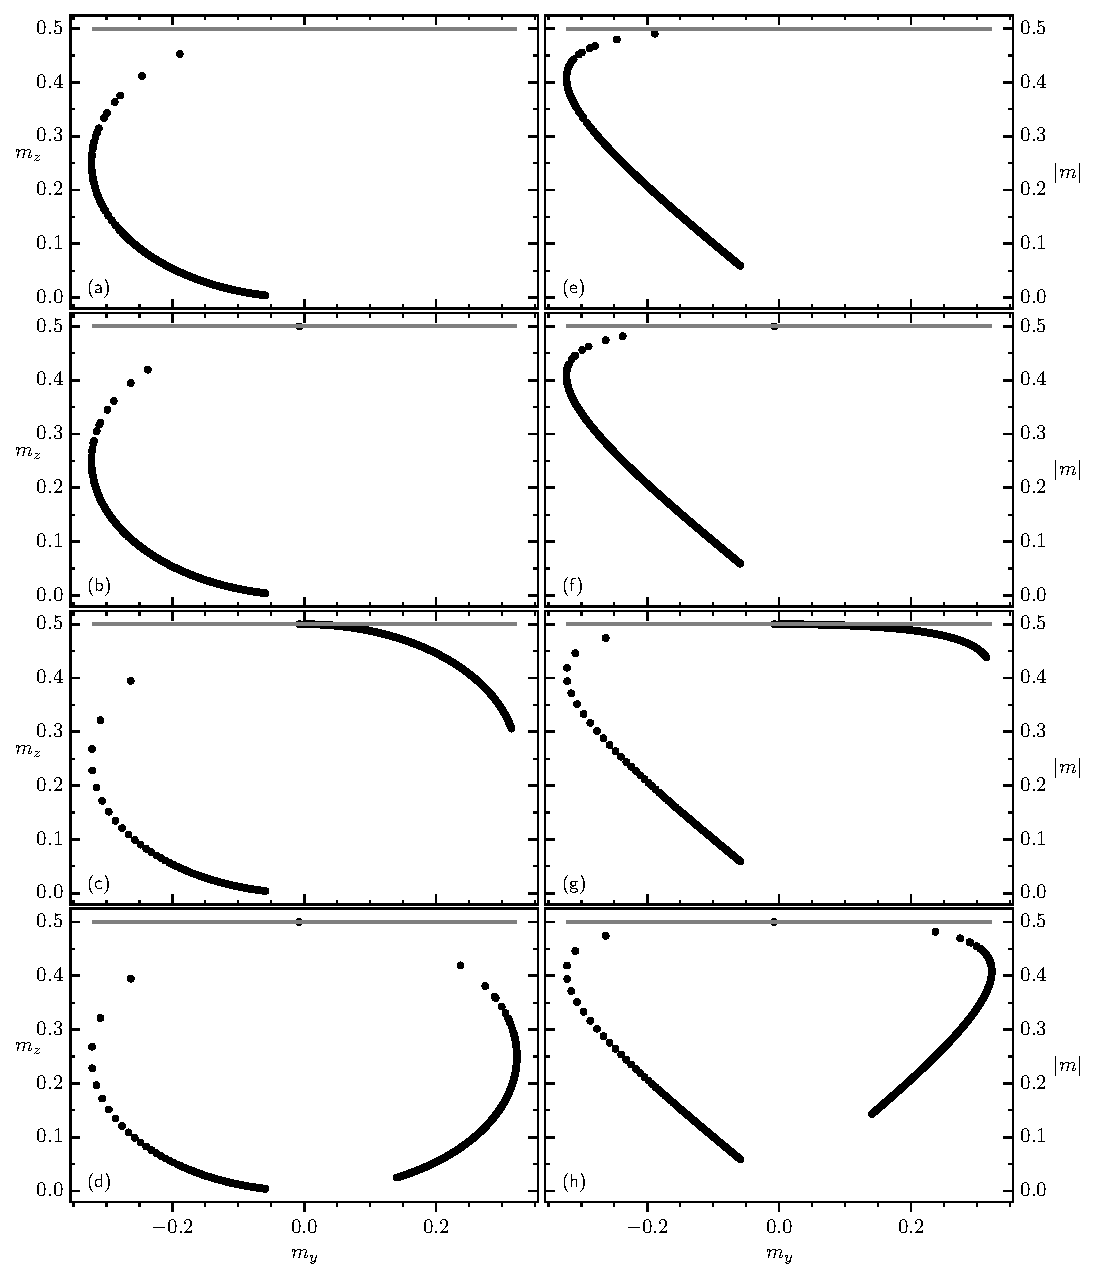
\includegraphics{pictures/fixp_boundaries.pdf}
        \caption{This graphic showes the range of $m_y$, $m_z$, $|m|$ for a parameter grid of $1.2\leq\kappa\leq24$ and $3\cdot10^{-7}\leq\omega\leq7$, $\Gamma=1$ $\gamma=0.2$. In the left column (a-d) the fixed points are shown in the $y-z$-plane, whereas in the right column (e-h) the modulus of the total angular momentum is depectid in dependence of $m_y$ for the different parameter values. The first row shows the fixed point in the parameter regime, where there is only one fixed point present. From the 2. row downwards the fixed points in the area of three stationary solutions are show in the order smallest, middle and largest $m_y$-value.}
    \end{figure}
    
    
    
    \section{Linearization eigenvalues for the unstable fixed points in the case $\delta=0$}
    \label{appendix:eig_del0}
    In this section of the appendix the eigenvalues of the linearization matrix for fixed points with middle and largest $y$-value are depicted. They show again their instability.
    \begin{figure}[H]
        \centering
        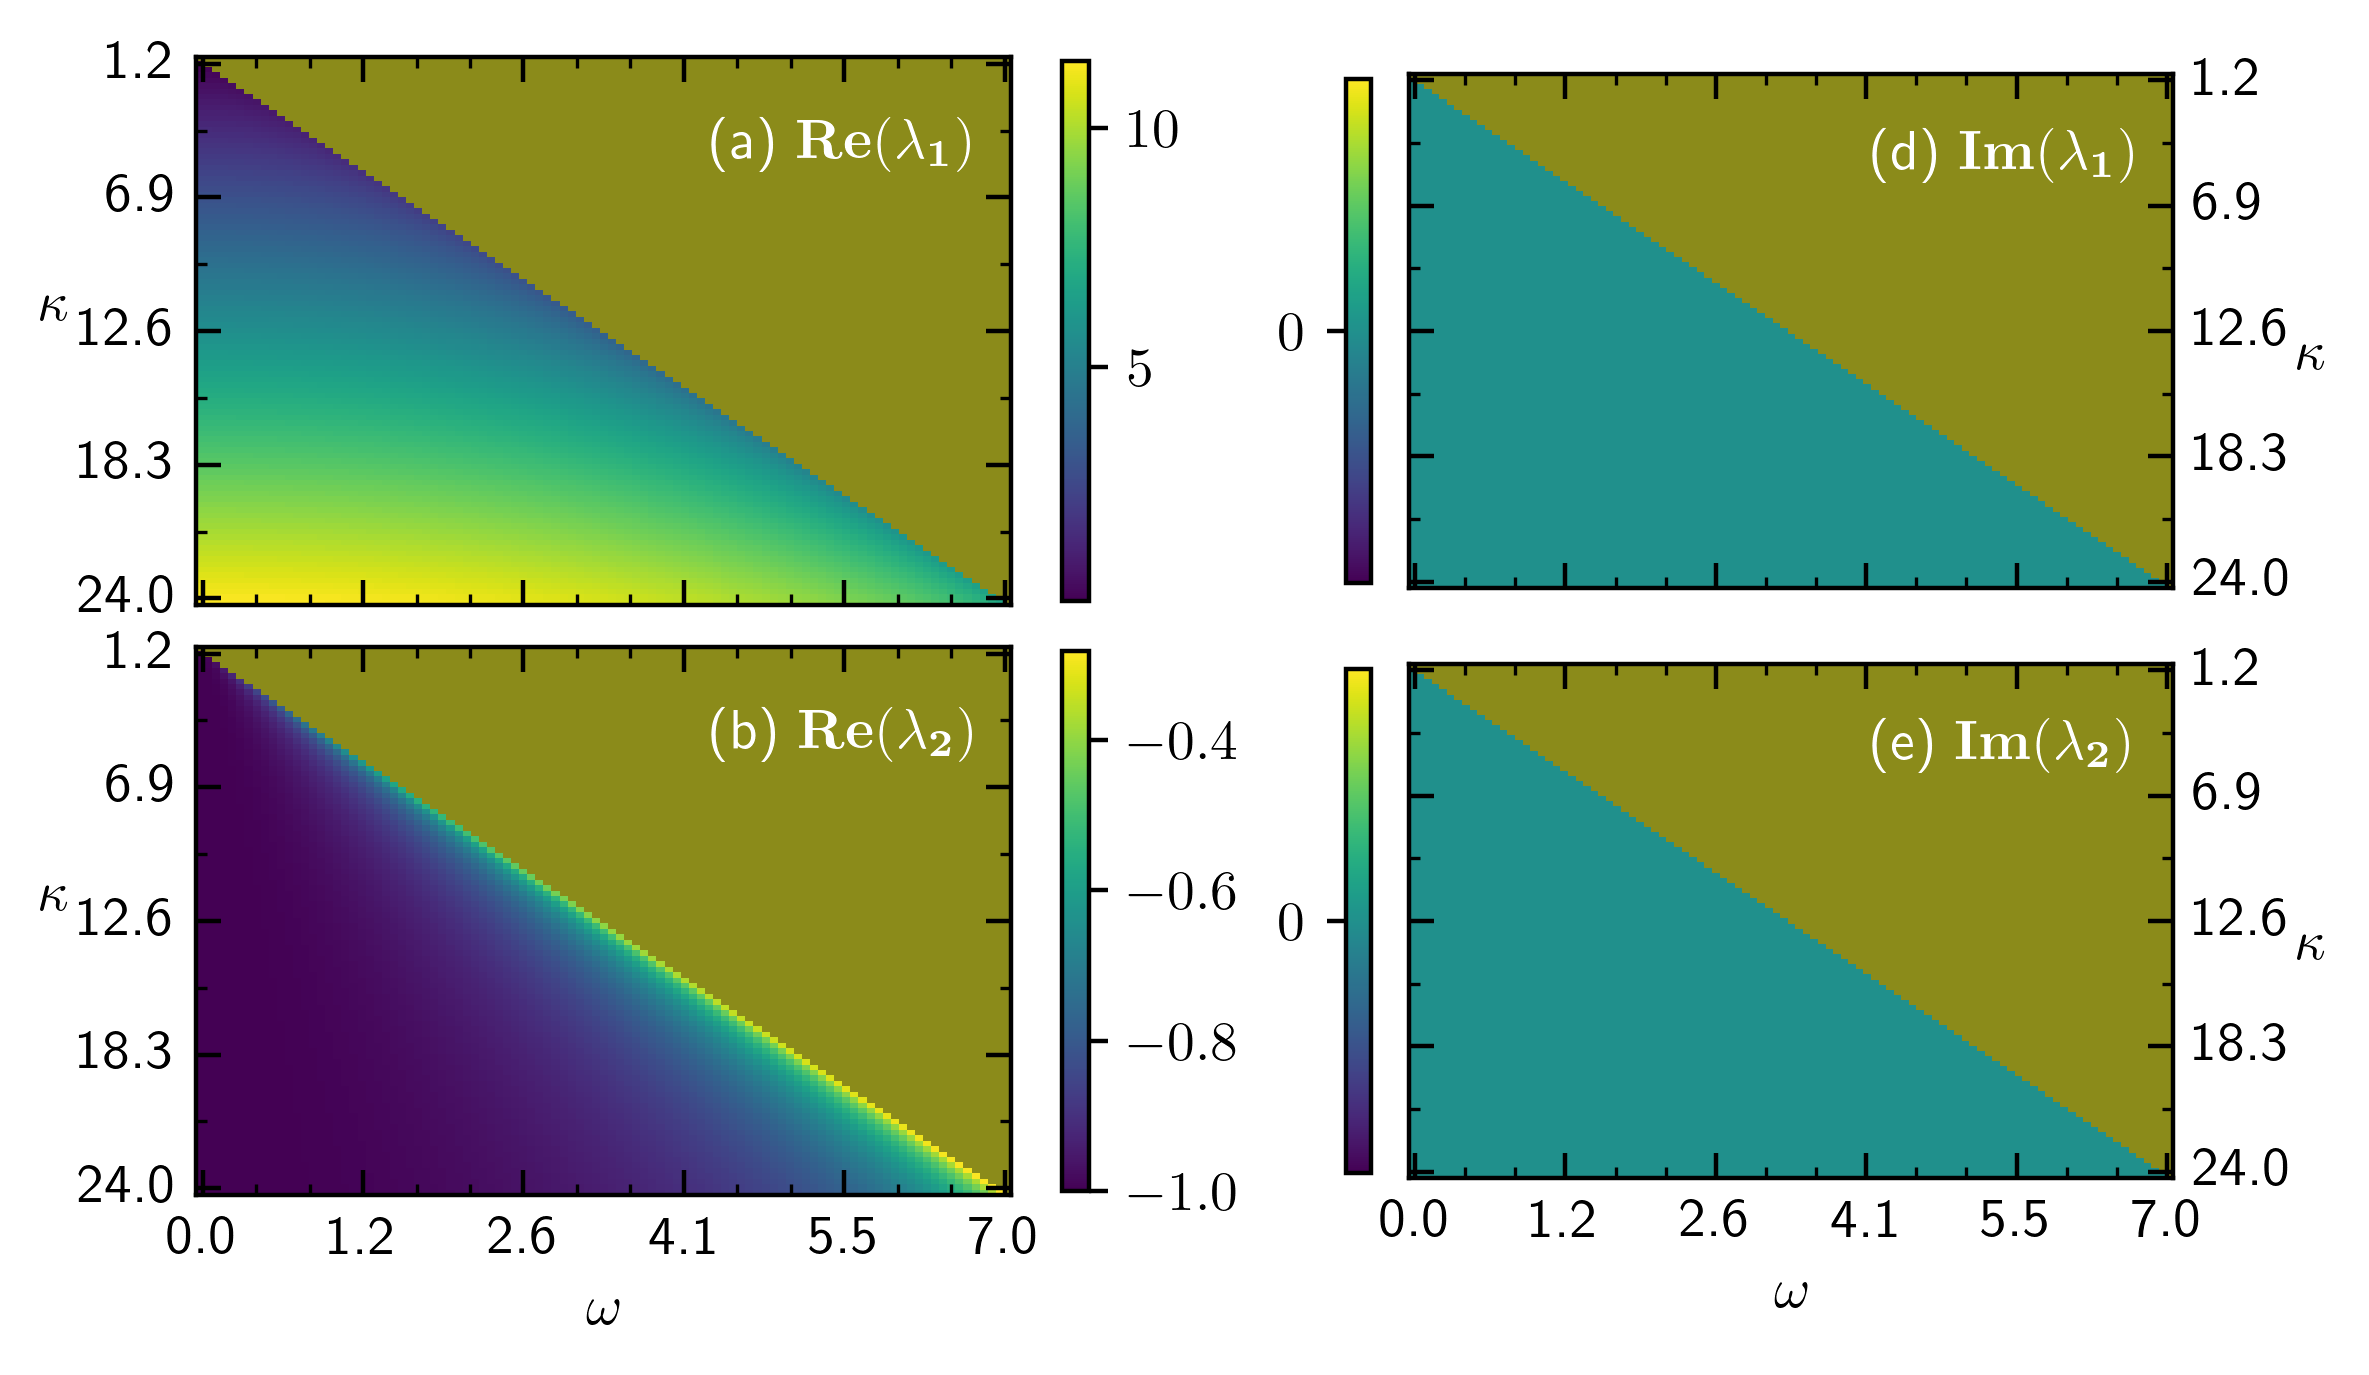
\includegraphics{pictures/lam_anal_m1.png}
        \caption{Real and imaginary part of the two of the eigenvalues of the linearization for the middle-$y$ stationary solution.
        }
    \end{figure}
    
    \begin{figure}[H]
        \centering
        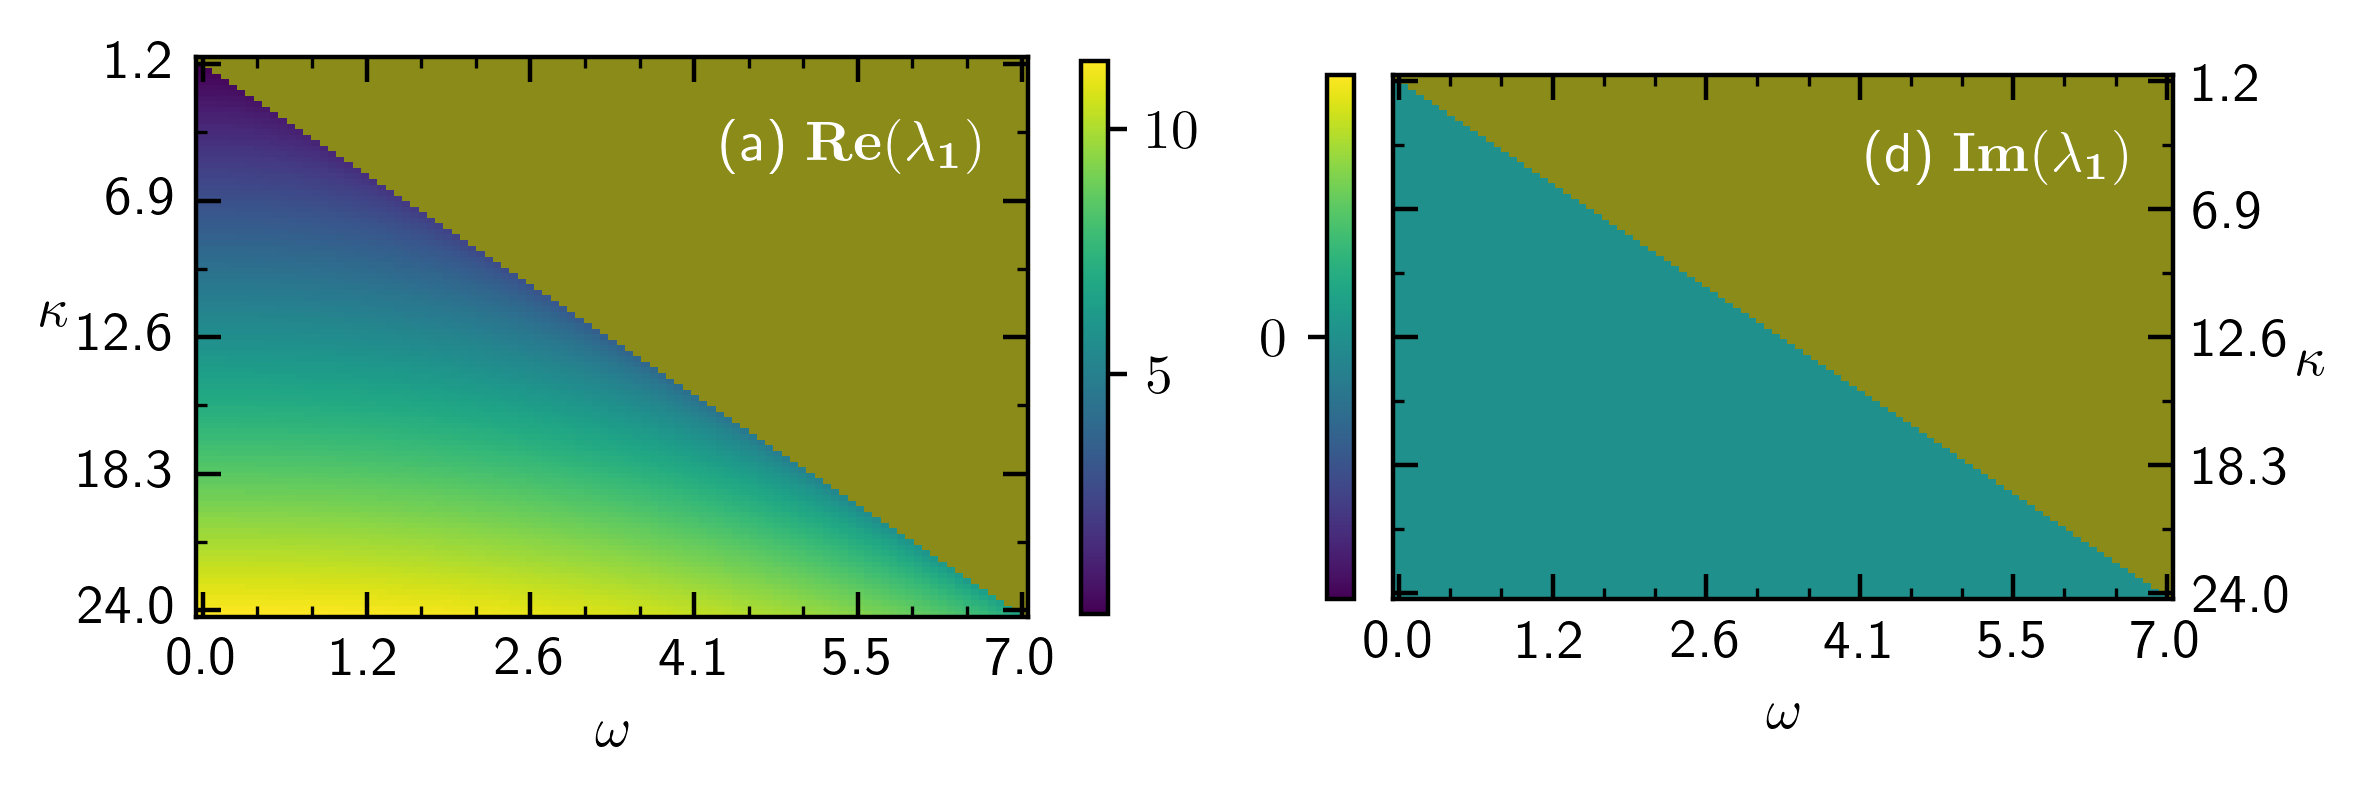
\includegraphics{pictures/lam_anal_m2.png}
        \caption{The remaining eigenvalue of the linearization for the the middle-$y$ stationary solution.
        }
    \end{figure}
    \begin{figure}[H]
        \centering
        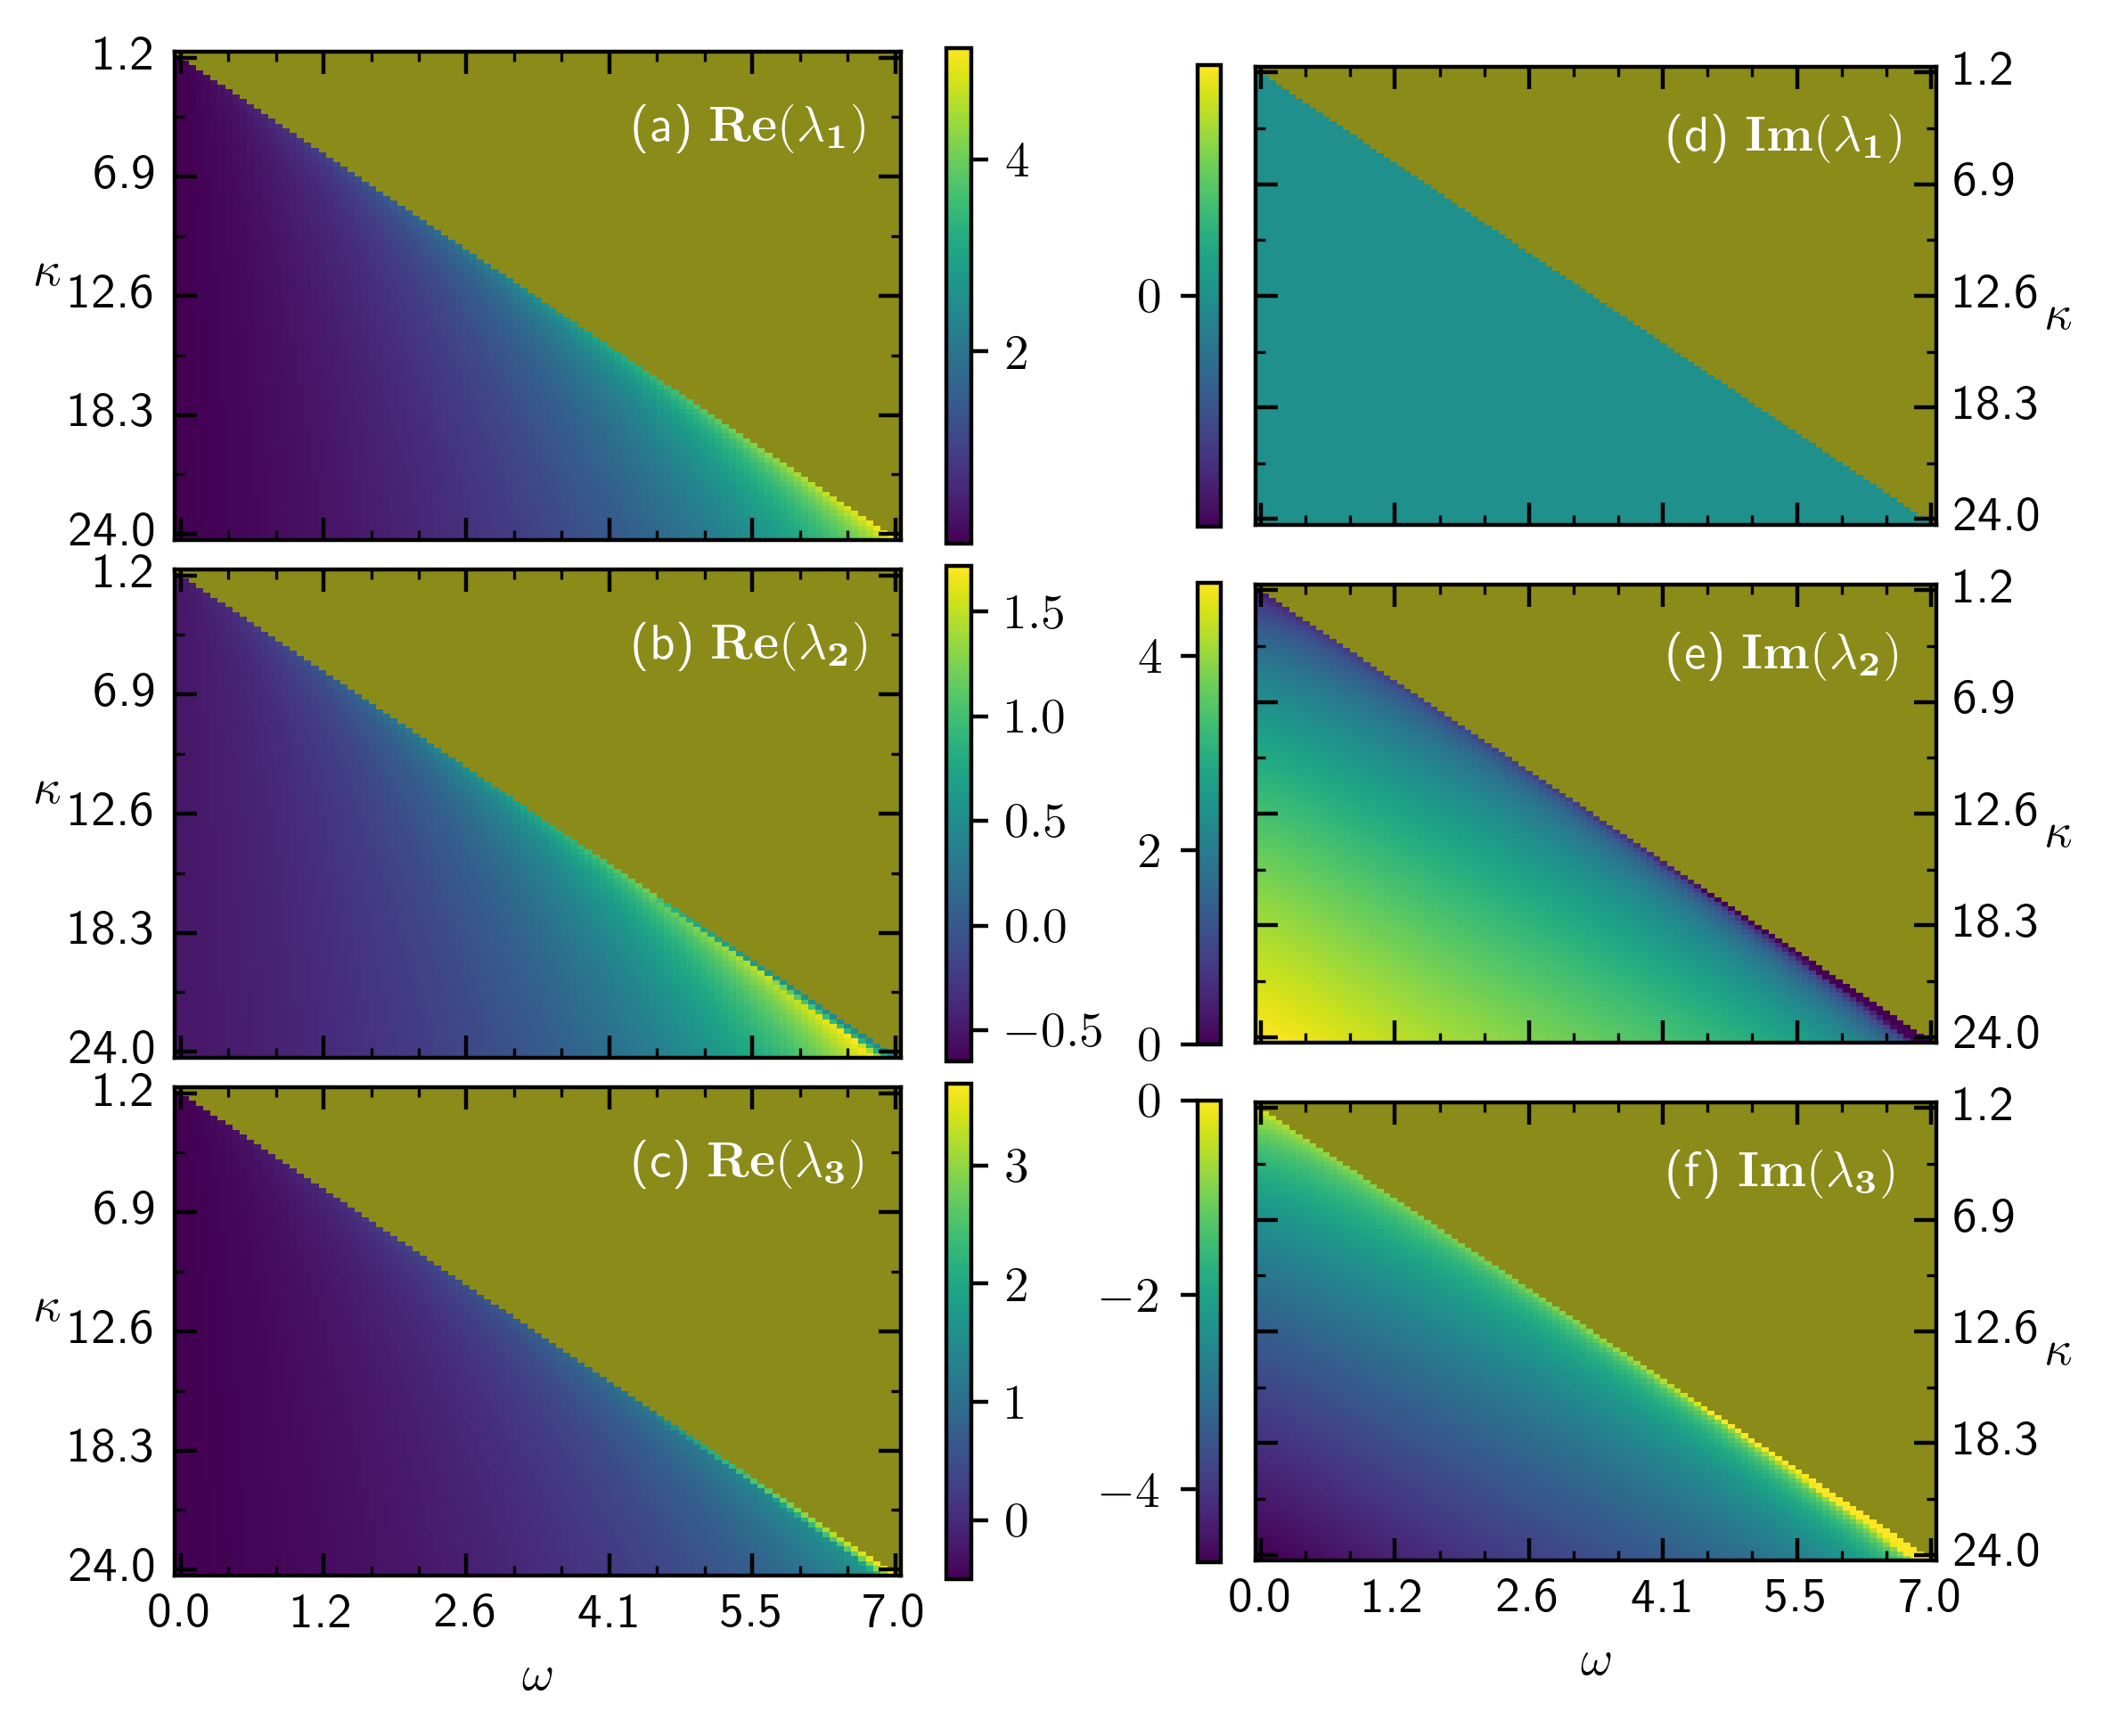
\includegraphics{pictures/lam_anal_l.png}
        \caption{Real and imaginary part of the eigenvalues from the linearization of the equations of motion are shown for the largest $y$-value fixed point.
        }
    \end{figure}
    
    \chapter{Appendix for the model with detuning}
    \section{Exemplary trajectories}
    \label{appendix:expl_traj}
    This paragraph shows a few exemplary long-time states of the system for the area where the transition of $m_x$-values is accompanied by multistability. Therefore I reconsider the outstanding regions in \figref{fig:fixedpoint_colormap} of \secref{sec:detuned_analysis}. I divide those regions into 9 parts and select randomly a parameter configuration out of those areas. For a few random initial conditions I depict the resulting long-time states.
    \begin{figure}[H]
        \centering
        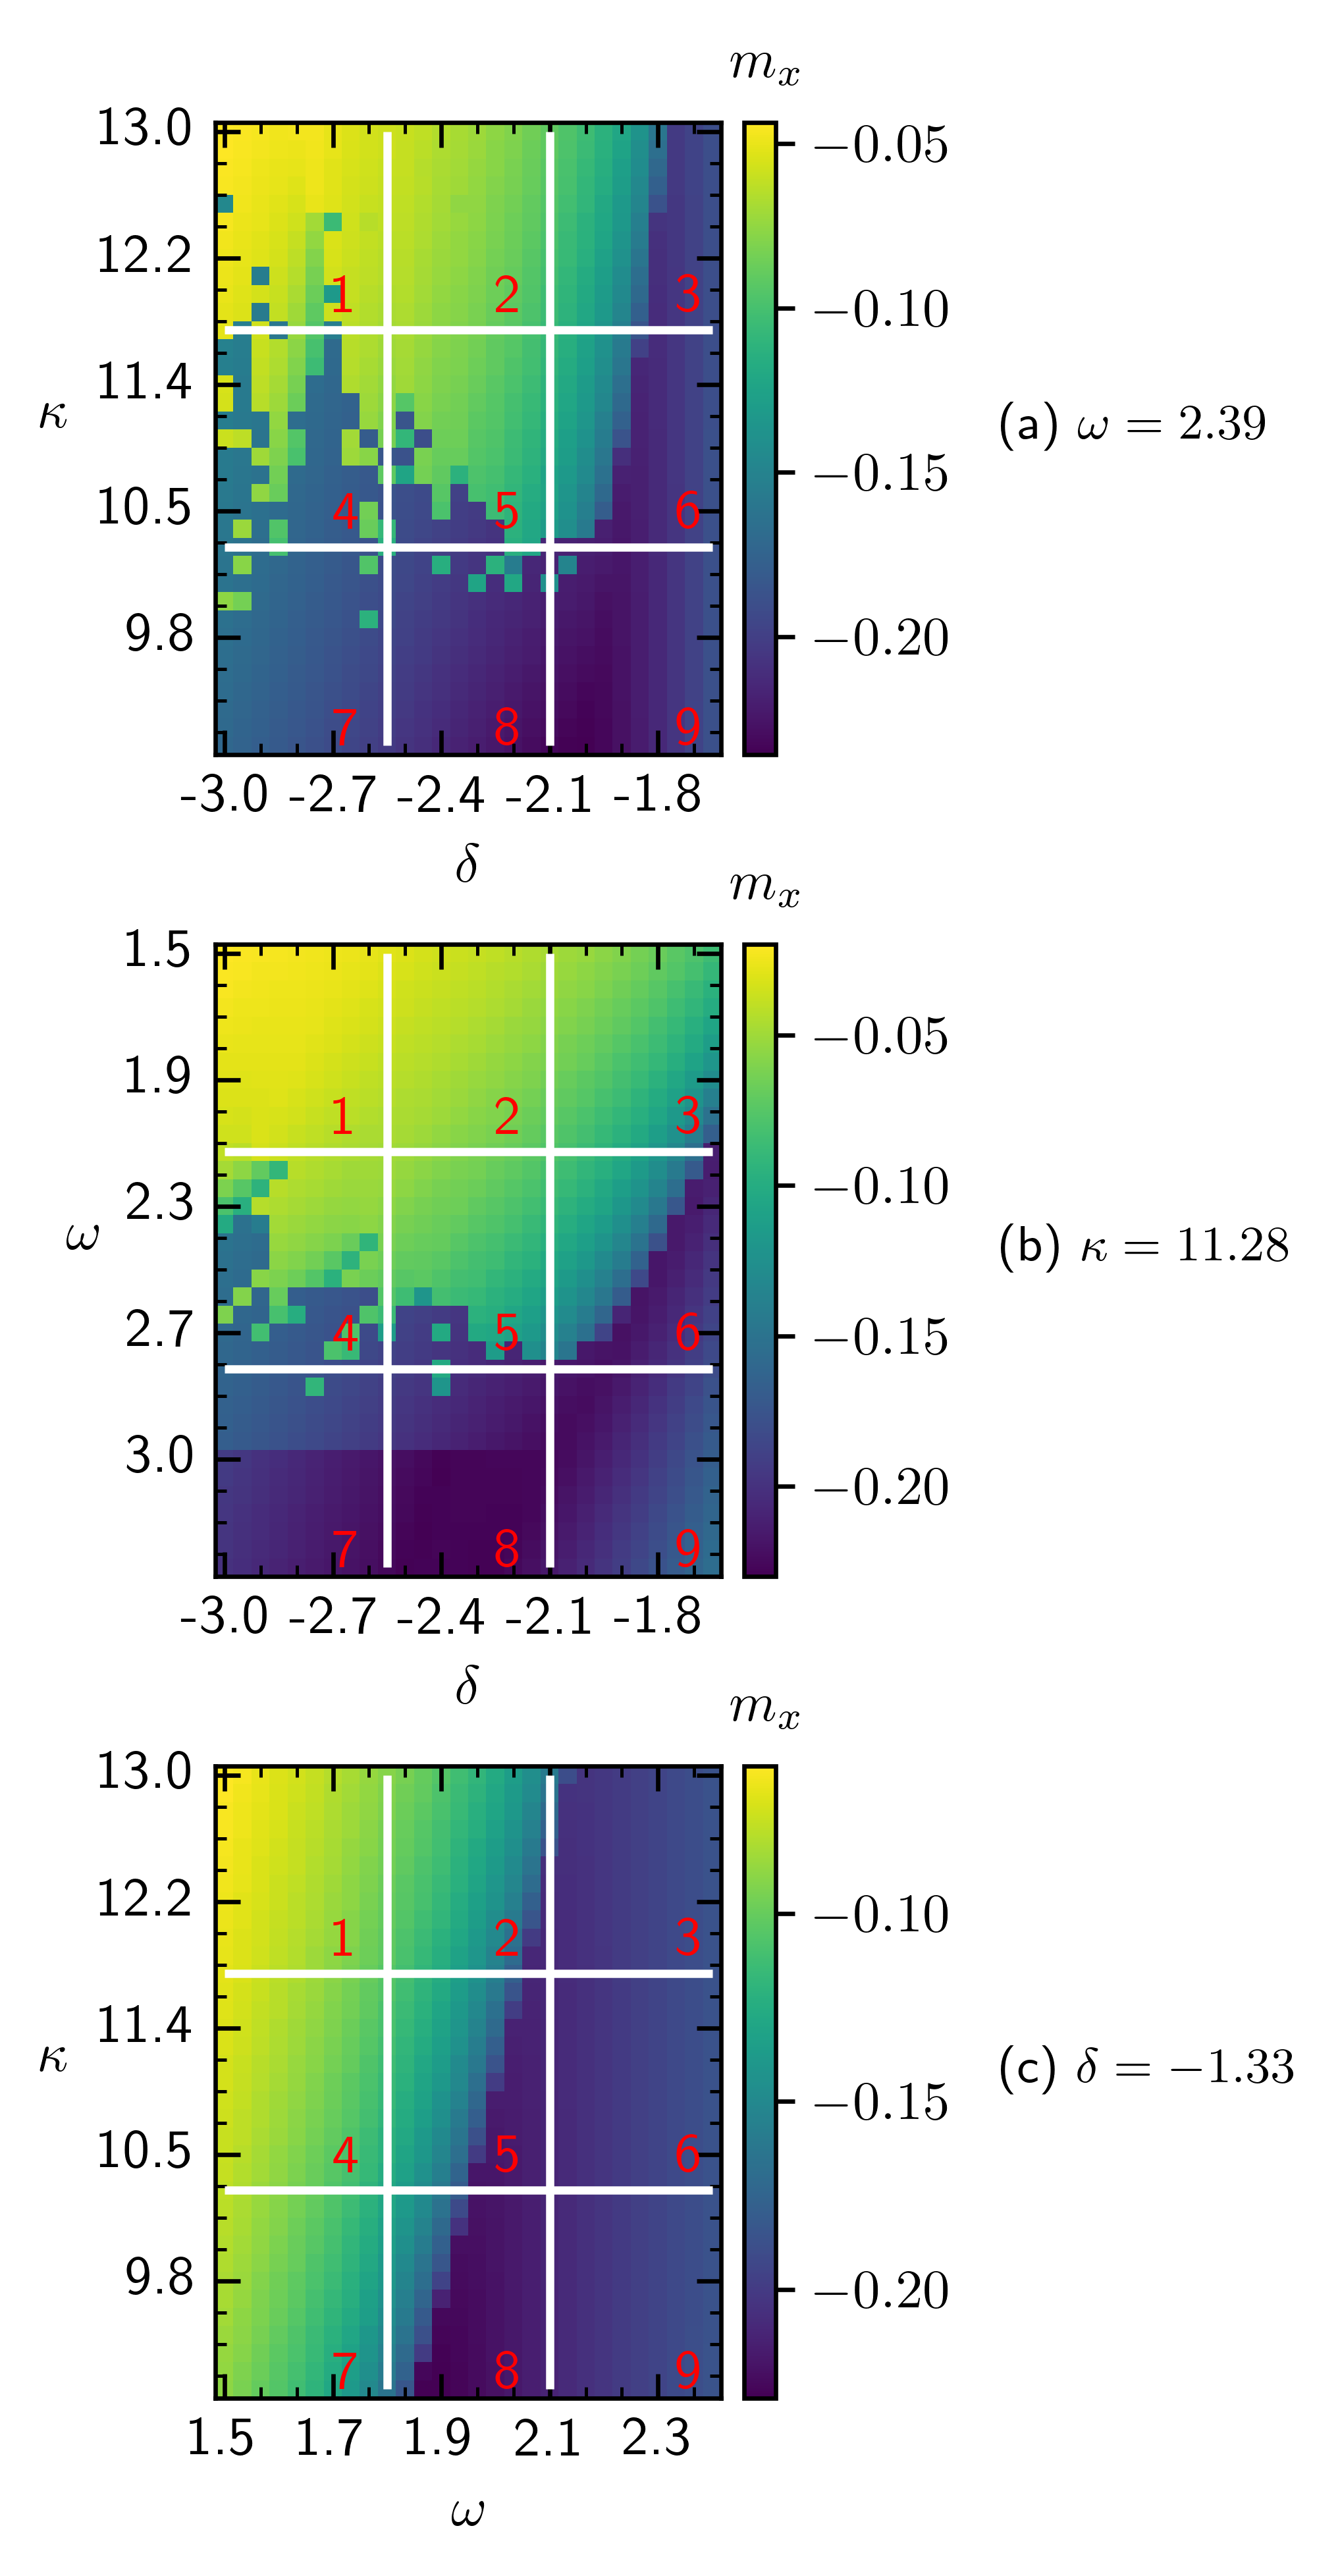
\includegraphics{pictures/combined_spec_sec.png}
        \caption{The division of the outstanding areas of \figref{fig:fixedpoint_colormap}.}
    \end{figure}
    
    \begin{figure}[H]
        \centering
        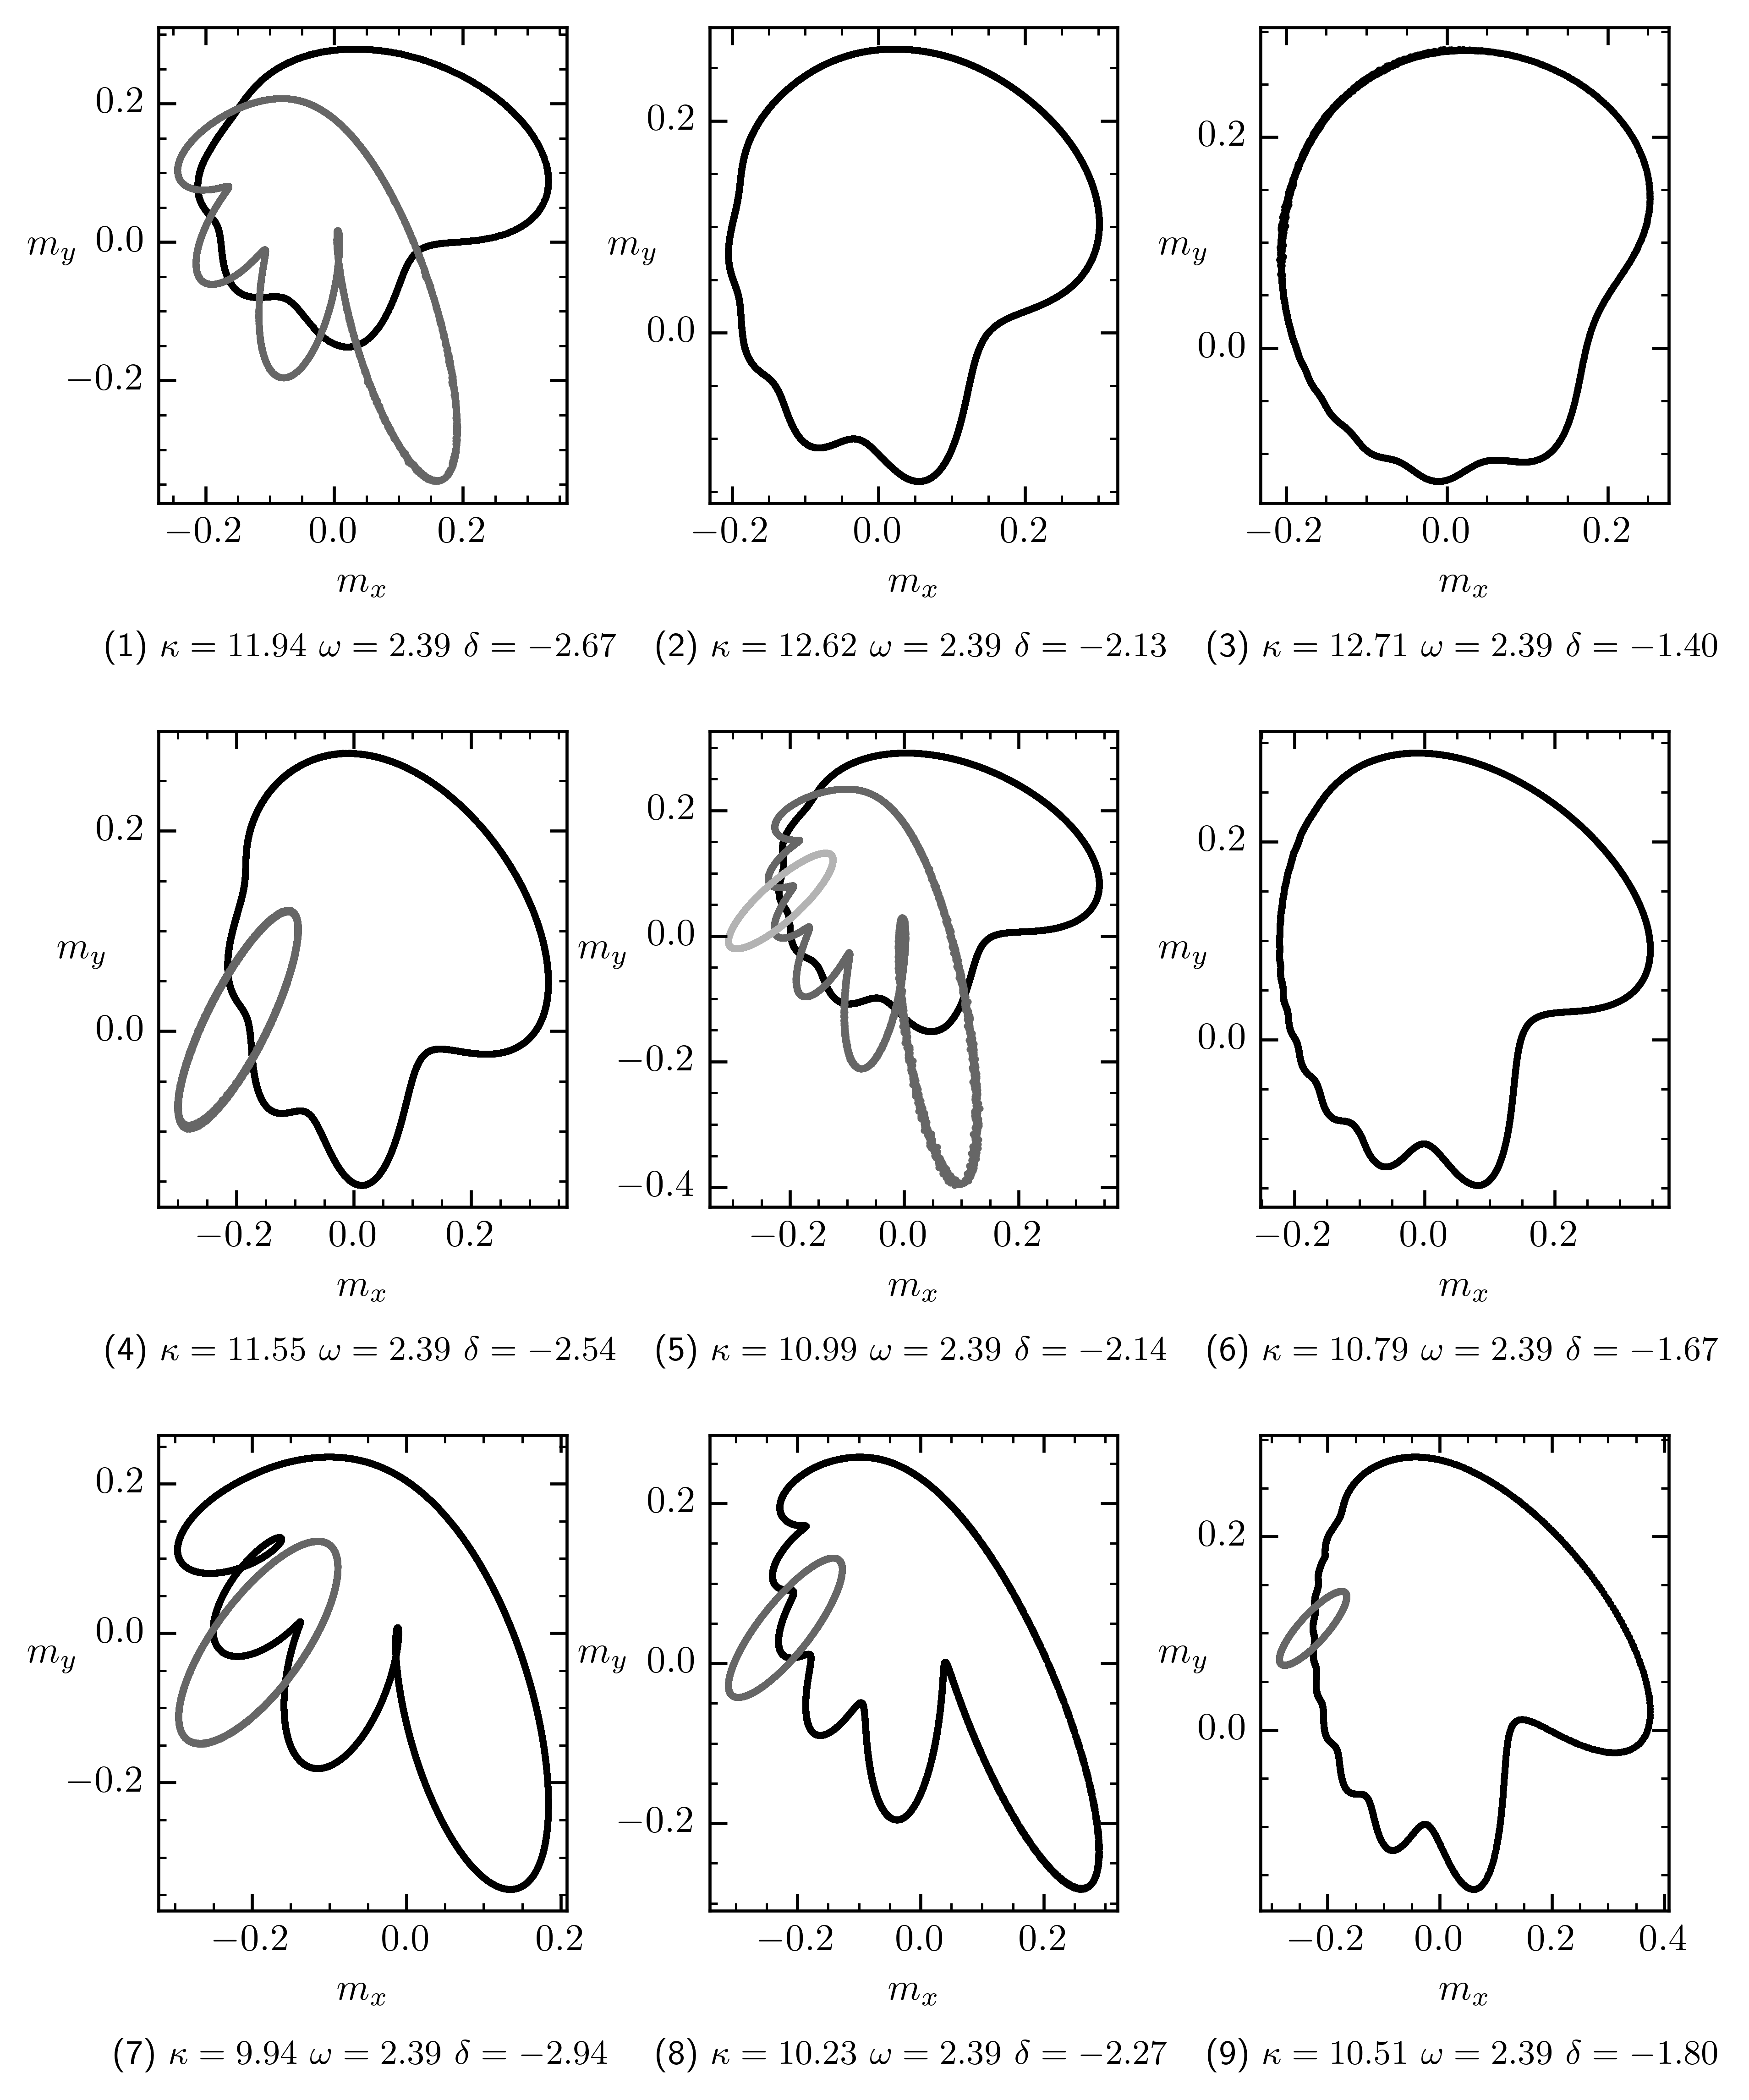
\includegraphics{pictures/lc_traj_wcut3.png}
        \caption{For $\omega=2.389$ possible long time states are shown for random values from the parameter grid. Where stationary points exist, I also drew the transition from the starting points to the stationary point.}
    \end{figure}
    
    \begin{figure}[H]
        \hspace*{-1cm}
        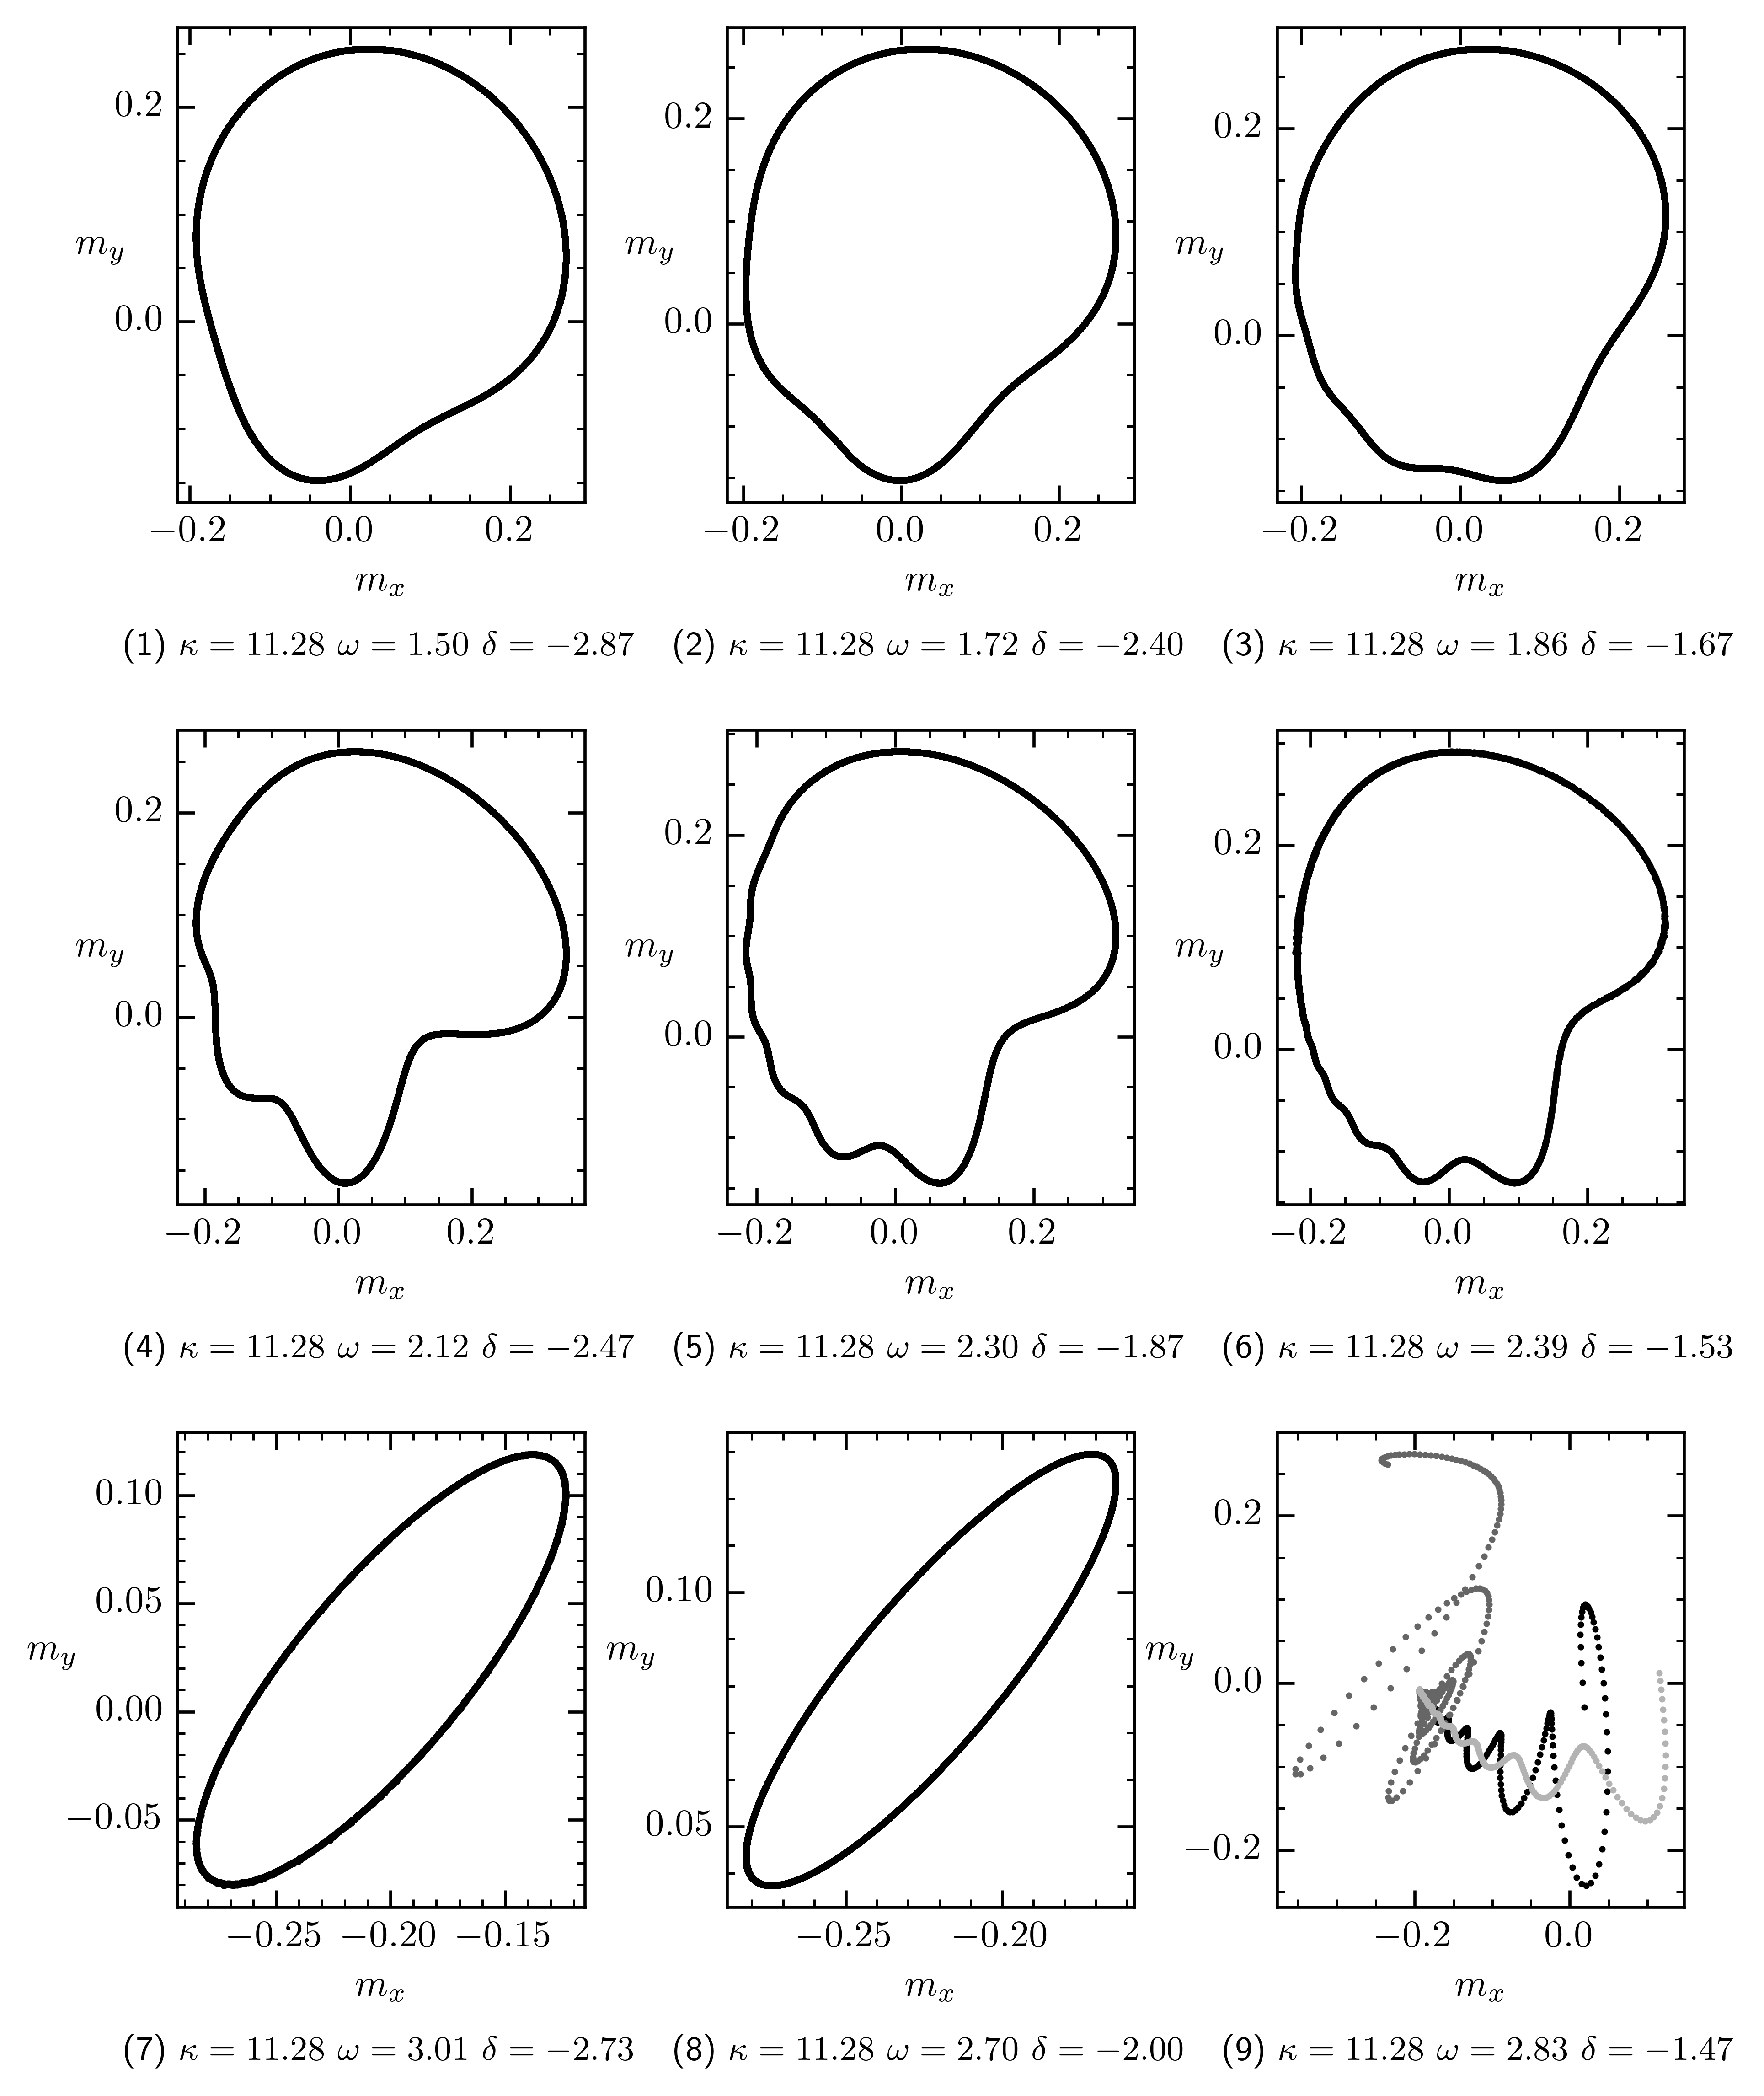
\includegraphics{pictures/lc_traj_kcut2.png}
        \caption{For $\kappa=11.28$ possible long time states are shown for random values from the parameter grid. Where stationary points exist, I also drew the transition from the starting points to the stationary point.}
    \end{figure}
    
    \begin{figure}[H]
        \centering
        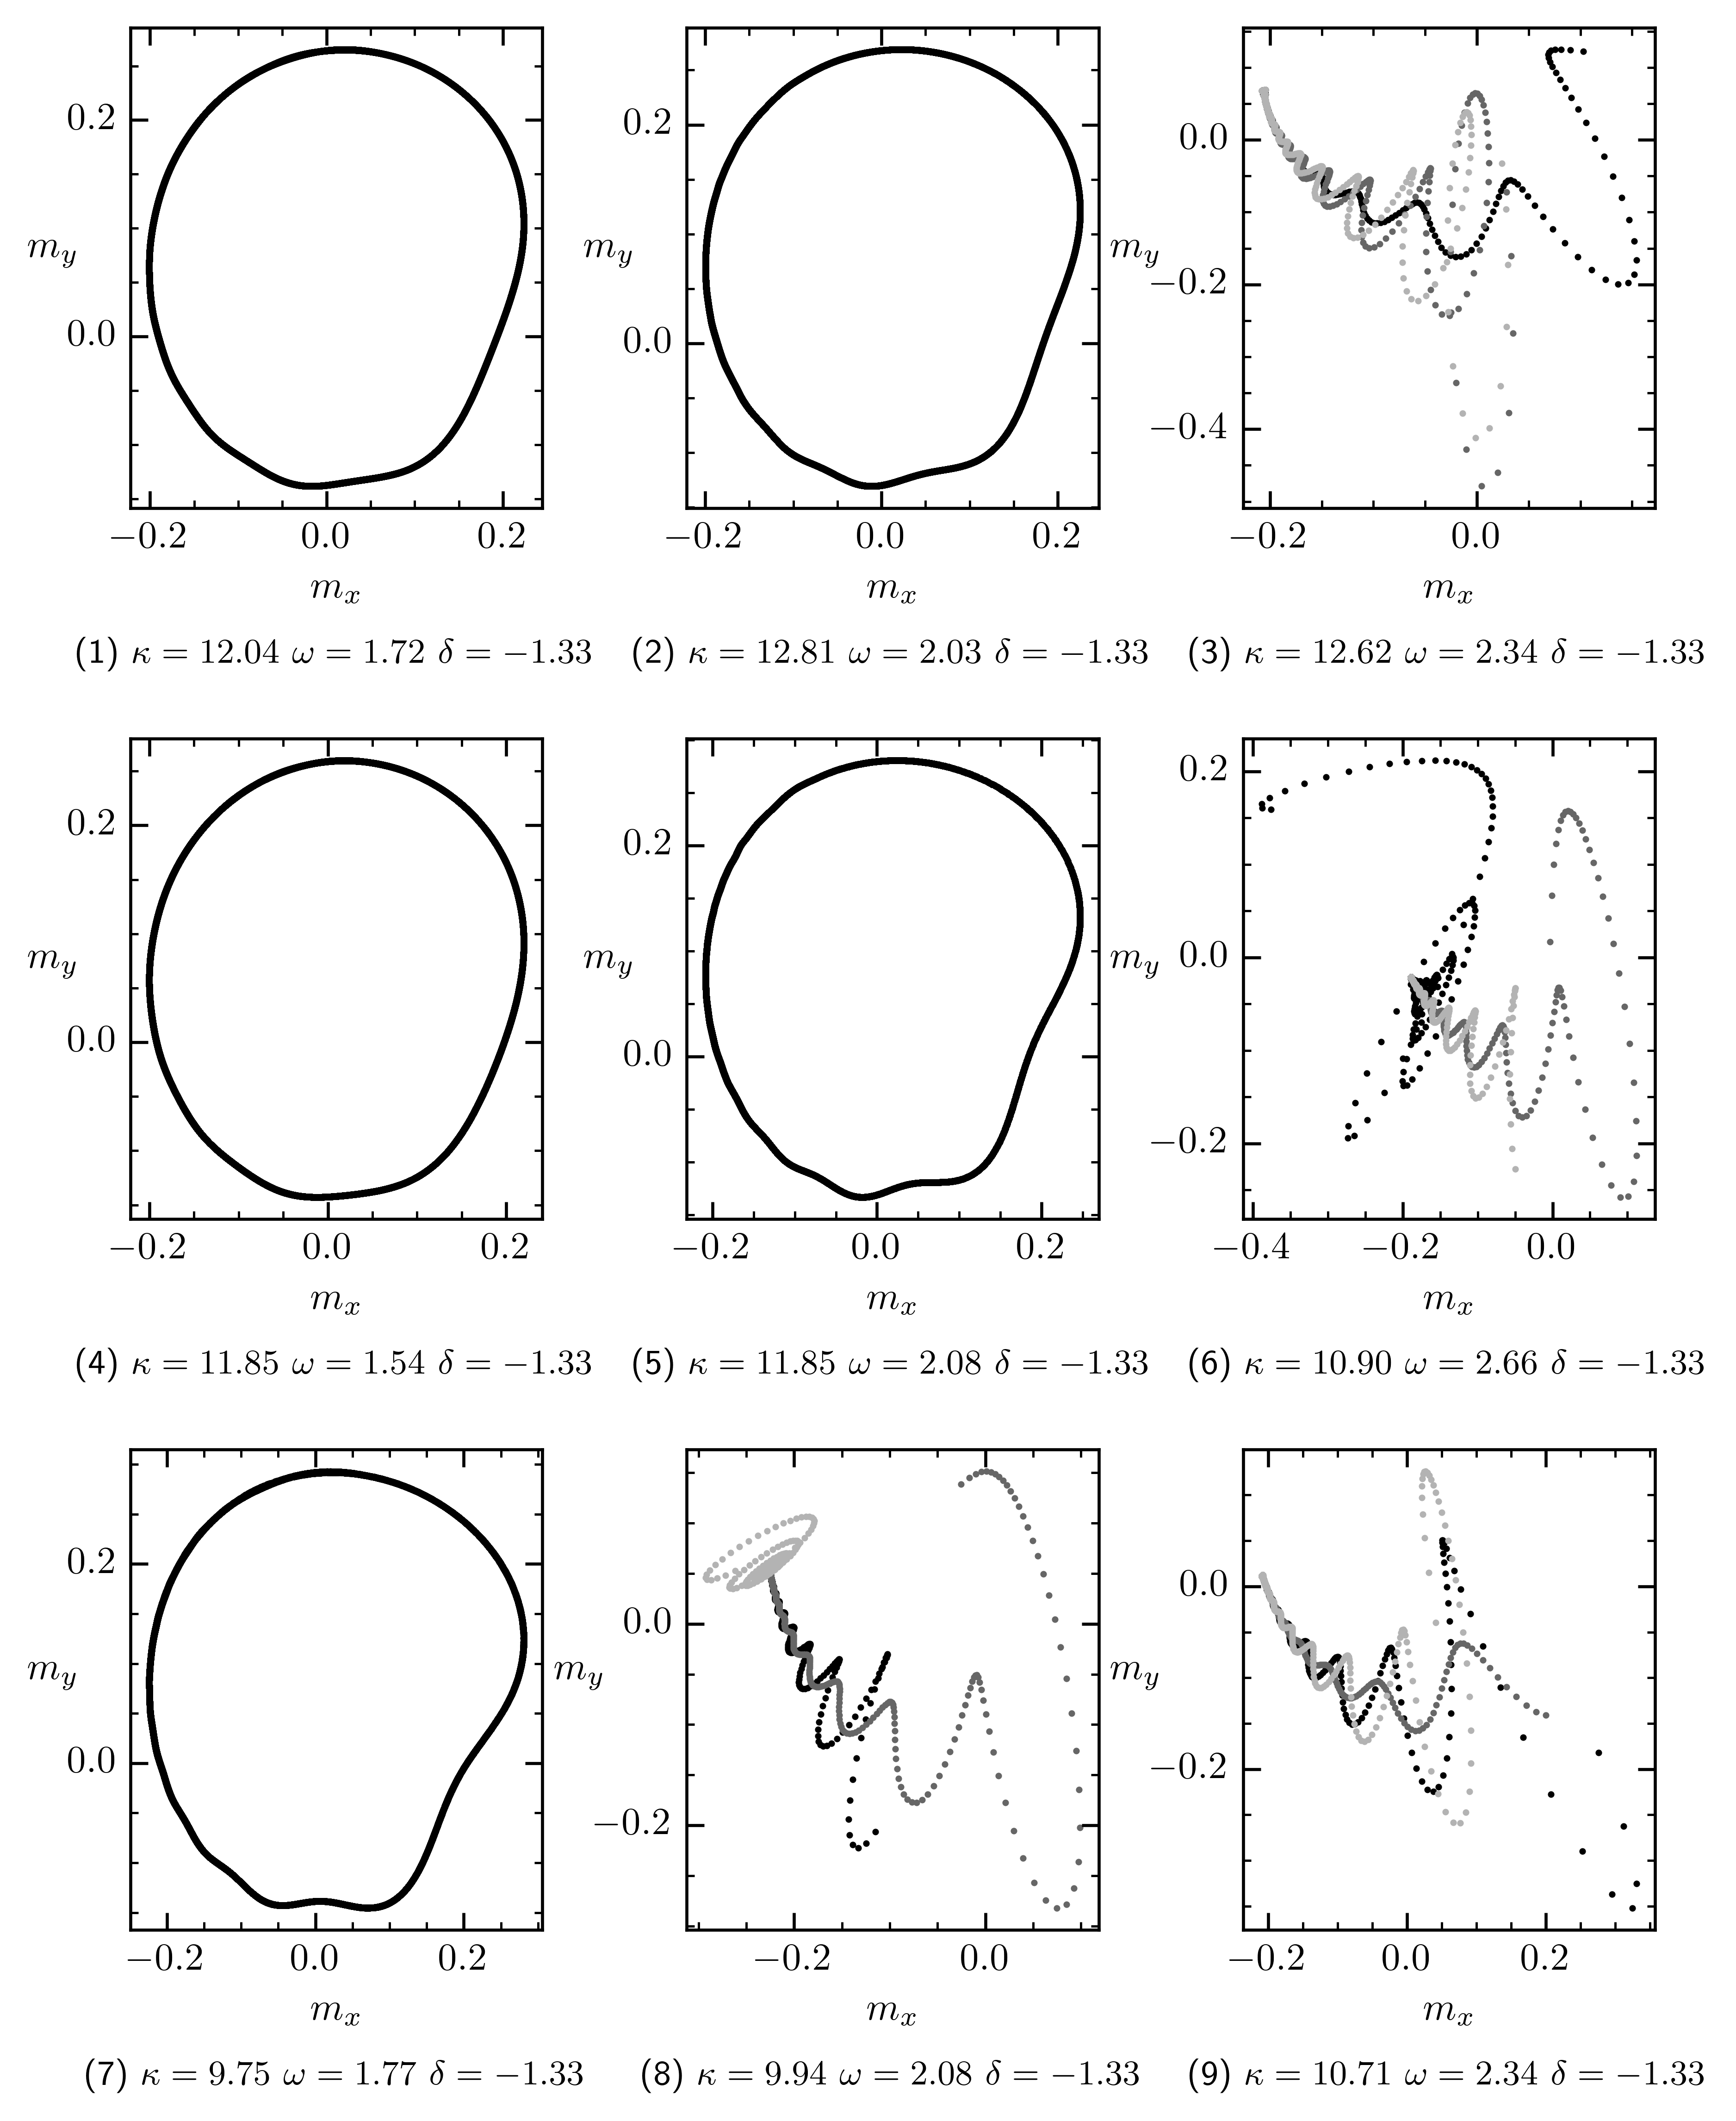
\includegraphics{pictures/lc_traj_dcut2.png}
        \caption{For $\delta=-1.33$ possible long time states are shown for random values from the parameter grid. Where stationary points exist, I also drew the transition from the starting points to the stationary point.}
    \end{figure}\newpage

    \section{Long-time states for varying dephasing strength}\label{app:gamma_analysis}
    An examination of the long-time states for different $\gamma$-values, which has been omitted in the main text, is briefly carried out at this point. For this purpose I again plot the stationary points as well as the average over a period of a limit cycle for different parameter values.
    \begin{figure}[H]
        \centering
        \caption{fixed points and averaged limit cycles over their period. In (a) $\gamma$ and $\delta$ are varied, while the other parameter a kept fixed. In (b) the cut with differing $\omega$ and $\delta$ is repeated for a different $\kappa$ and more importantly a different $\gamma$ value. $\Gamma=1$ as always. The white dashed line separates the region of limit cycles from that where stationary points exist. In both plots the area above the white line is the time crystal phase.}
        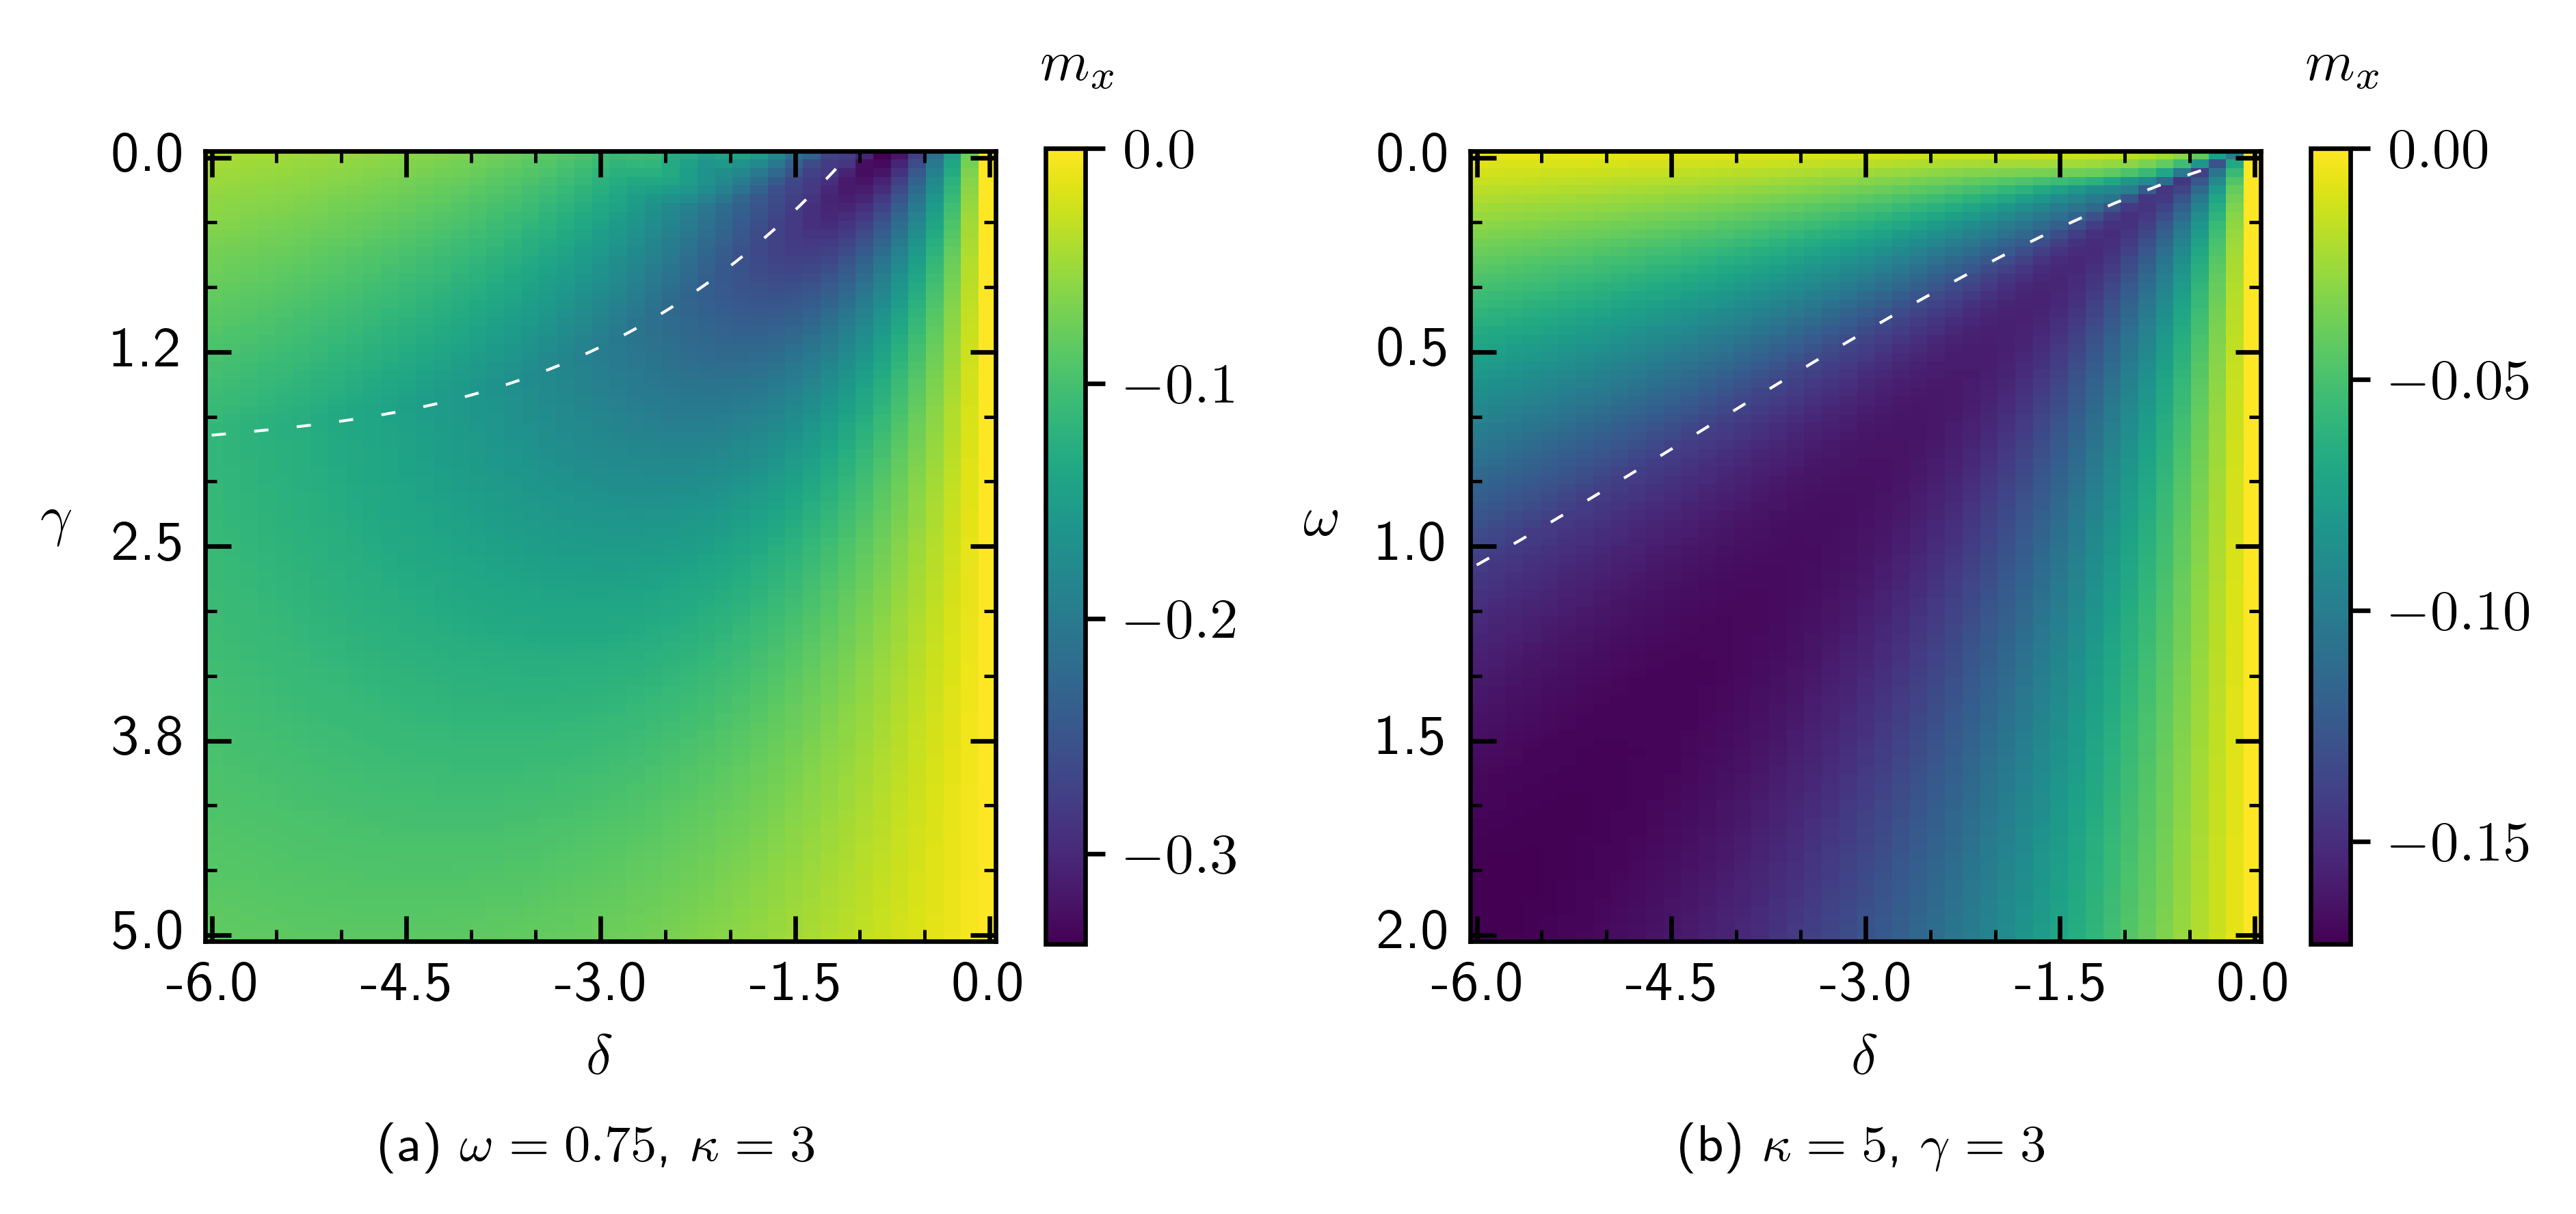
\includegraphics{pictures/limit_cycle_mean_gw.png}
        \label{fig:gamma_longtime}
    \end{figure}
    A several interesting observations can be made. Starting with \figref{fig:gamma_longtime}(b) one can see that the phase separation line has qualitatively the same shape as for $\gamma=0.2$. It again follows the property of synchronization effects that the larger the detuning between the considered systems is the larger the coupling between them has to be in order to see synchronization. I can also inform the reader that the parameter set that has been chosen in \figref{fig:gamma_longtime}  exhibits no multistability. For all configuration only one limit cycle or one stationary solution exists. \\
    What can be additionally observed is that the long-time states show a valley of small $m_x$ values, that lies near the phase separation line but does not coincide with it. \\\\
    Turning to \figref{fig:gamma_longtime}(a) one finds that the time crystal phase is stable for a wide range of dephasing strength for certain parameter constellations. What is also intriguing is that the higher $\gamma$ is the larger, in absolute value, the detuning has to be in order to observe a time crystal phase. The form of the phase separation line also suggests that there might be a maximal value of dephasing such that above that value no limit cycles can arise. But this definitively has to be yet verified, what could be an interesting subject of future analysis.




% \end{appendices}